\chapter{Neuro-Symbolic Verification of Safety Critical Systems}
\label{chap:ansya}

Formal verification is a collection of symbolic techniques aimed at proving the correctness of a system with respect to some specification. Although extremely important for domains such as Safety-critical Systems, verification is an expensive process, often intractable for larger instances. Moreover, the fully-symbolic nature, makes (sub-symbolic) perception a blind spot of formal verification. In this chapter we employ the \textsc{LTLZinc-Safety} datasets to explore a simple Neuro-symbolic approach to efficiently approximating the verification process by means of Sequence Classification, while preserving the ability to adapt to perceptual stimuli.
%
The content of this chapter is a significant extension of our ANSyA2025 workshop paper~\cite{lorello2025ansya}.

\section{Background}
Safety-critical Systems are domains in which failure might produce significant damage to the system itself or to the environment, or even loss of life~\cite{knight2002safety}. Typical application areas include healthcare, for critical tasks such as the monitoring of biomedical devices~\cite{vakhter2022threat}, transportation, as in the case of aircraft flight control systems~\cite{stolzer2023safety}, or space missions, for the detection of anomalies and cyber-security vulnerabilities~\cite{vessels2019cybersecurity}. In most of these scenarios, safety must be ensured by assessing that the behavior of the system is compliant with strict constraints, such as time constraints (e.g., tasks that must complete their executions within certain time limits) or logic constraints (e.g., events that must occur in a predefined sequential order)~\cite{graydon2014realistic,favaro2018application}. Many formalisms can be used to model these systems, such as Stochastic Time Petri nets~\cite{carnevali2012quantitative}, Deterministic or Symbolic Finite-state Automata~\cite{giantamidis2020efficient}, Linear Temporal Logic (\LTL)~\cite{ma2010approach}, Fault Trees~\cite{roth2013modeling,ruijters2015fault} and others, with the aim of quantitatively evaluating  dependability attributes~\cite{maurya2020reliability,carnevali2025faultflow}.
In this chapter we explore the possibility of casting the problem of verification of Safety-critical Systems into an \textsc{LTLZinc} problem. 
%
Consider, for instance, a Safety-critical System composed of two devices ($A$ and $B$) characterized by ten possible states $\gY \in [0, 9]$, each associated with a perceptual signature, in the form of audio spectrograms $\mathcal{X} \in \left\{\mathimg{urban_0.png}, \ldots, \mathimg{urban_9.png}\right\}$. Suppose this system must comply to a \textit{liveness} property~\cite{alpern1985defining} $\gF$, asserting that an event $p$ (``the sensor is in state 4'') registered by sensor $A$ must always be followed by another event $q$ (``the sensor is in state 7''), observed by sensor $B$. Events can be tracked, by systematically evaluating the validity of a set of relational predicates $\mathcal{C}$, on the state of the system over time.
The behavior described above can be represented compactly by the following \textsc{LTLZinc} specification:
\begin{align*}
	\begin{split}
		\mathcal{X}\colon & A, B = \left\{\mathimg{urban_0.png}, \mathimg{urban_1.png}, \mathimg{urban_2.png}, \mathimg{urban_3.png}, \mathimg{urban_4.png}, \mathimg{urban_5.png}, \mathimg{urban_6.png}, \mathimg{urban_7.png}, \mathimg{urban_8.png}, \mathimg{urban_9.png}\right\}\\
		\mathcal{Y}\colon &A, B = [0, 9]\\
		\mathcal{C}\colon &\texttt{p}(Z): Z = 4, \\
		& \texttt{q}(Z): Z = 7\\
		\mathcal{F}\colon & \ltlglobally (\texttt{p}(A) \rightarrow \ltlfinally \texttt{q}(B)).
	\end{split}
\end{align*}
In this setting, the verification of traces of events generated by the Safety Critical System, can be cast into a Sequence Classification with background knowledge setting, and addressed by the same Neuro-symbolic pipeline introduced in Chapter~\ref{chap:ltlzincseq}.
%
\textsc{LTLZinc} enables the design of experiments in different learning and reasoning scenarios, depending on what kind of knowledge is available at training time, and which element of the tuple  $\langle \gX, \gY, \gC, \gF \rangle$ constitutes the learning objective. For example, in many cases, a Safety-critical System is designed with predefined specifications in mind, and it is therefore reasonable to assume prior knowledge about both $\gC$ and $\gF$, but not the mapping $\gX \mapsto \gY$.
%Within this setting, a \textit{sequence classification} task corresponds to predict whether a given sequence of perceptual stimuli $\gX^{(t)}$ along a discrete set of $n$ time-steps $t = \{1, \ldots, n\}$ satisfies $\gF$ or not,  and it corresponds to the \textit{verification} of $\mathcal{F}$ within a given sequence $\mathcal{X}^t$, by neuro-symbolic means. 
In other cases, either $\mathcal{C}$ or $\mathcal{F}$ could be unknown, and the sequence classification task would thus involve the \textit{induction} of temporal safety properties directly from system traces: in these settings, the Neuro-symbolic system is trained to discriminate between positive and negative sequences, without knowing neither $\gF$ nor $\gC$.

\section{Experiments}
We perform experiments on \textsc{LTLZinc-Safety-Prop} and \textsc{LTLZinc-Safety-FOL} by employing the modular pipeline described in Chapter~\ref{chap:ltlzincseq}.
As the perceptual component of \textsc{LTLZinc-Safety} is significantly more challenging than the one of \textsc{LTLZinc-Sequential}, we replace the \textsc{ic} module with a ResNet18~\cite{he2016deep}, pre-trained on ImageNet. 
Images are augmented during training and inference, according to the original ResNet18 transforms.
The \textsc{cc} and \textsc{nsp} modules are jointly initialized in two flavors: (i.) \textit{Symbolic} (Problog \textsc{cc}, Fuzzy \textsc{nsp}), and (ii.) \textit{Neural} (MLP-L \textsc{cc}, GRU-L \textsc{nsp}).
%
After selecting optimal hyper-parameters (optimizer: Adam, learning rate: $10^{-4}$) on a simplified task (the one introduced at the beginning of the chapter), we initialize the \textsc{IC} module with one epoch of pre-training on image labels only, then provide supervisions at every stage ($\lambda_{\textsc{CC}} = \lambda_{\textsc{NSP}} = \lambda_{\textsc{SC}} = 1.0, \lambda_\textsc{IC} = 0.1$). For either dataset, we perform two batches of experiments, to assess the effect of training budget: (i.) \textit{low training budget} (1 epoch of training), and (ii.) \textit{high training budget} (7 epochs of training).

\paragraph{Results on \textsc{LTLZinc-Safety-Prop}.}
\begin{table*}[!t]
	\centering
	\resizebox{\textwidth}{!}{
		\begin{tabular}{cccccccc}
			\toprule
			\multirow{2}{*}{\sc Task} & \multirow{2}{*}{\sc Category} & \multirow{2}{*}{\shortstack[c]{\sc Best Epoch}} & \multirow{2}{*}{\shortstack[c]{\sc Average\\\sc Accuracy}\raisebox{1ex}{\:$\uparrow$}} & \multirow{2}{*}{\shortstack[c]{\sc Label\\\sc Accuracy}\raisebox{1ex}{\:$\uparrow$}} & \multirow{2}{*}{\shortstack[c]{\sc Constraint\\\sc Accuracy}\raisebox{1ex}{\:$\uparrow$}} & \multirow{2}{*}{\shortstack[c]{\sc Successor\\\sc Accuracy}\raisebox{1ex}{\:$\uparrow$}} & \multirow{2}{*}{\shortstack[c]{\sc Sequence\\\sc Accuracy}\raisebox{1ex}{\:$\uparrow$}}\\
			& & & & & & & \\
			\midrule
			\multirow{2}{*}{Task 1} & Symbolic & $0$ & $\textbf{0.67} $ {\tiny ($\pm 0.03$)} & $\textbf{0.72} $ {\tiny ($\pm 0.02$)} & $\textbf{0.82} $ {\tiny ($\pm 0.02$)} & $\textbf{0.58} $ {\tiny ($\pm 0.05$)} & $\textbf{0.55} $ {\tiny ($\pm 0.06$)}\\
			& Neural & $1$ & $0.61 $ {\tiny ($\pm 0.00$)} & $0.69 $ {\tiny ($\pm 0.02$)} & $0.78 $ {\tiny ($\pm 0.02$)} & $0.44 $ {\tiny ($\pm 0.00$)} & $0.52 $ {\tiny ($\pm 0.05$)}\\
			\hdashline
			\multirow{2}{*}{Task 2} & Symbolic & $0$ & $\textbf{0.65} $ {\tiny ($\pm 0.03$)} & $\textbf{0.70} $ {\tiny ($\pm 0.05$)} & $\textbf{0.81} $ {\tiny ($\pm 0.05$)} & $0.57 $ {\tiny ($\pm 0.03$)} & $0.51 $ {\tiny ($\pm 0.01$)}\\
			& Neural & $1$ & $\textbf{0.65} $ {\tiny ($\pm 0.05$)} & $0.62 $ {\tiny ($\pm 0.06$)} & $0.77 $ {\tiny ($\pm 0.04$)} & $\textbf{0.61} $ {\tiny ($\pm 0.10$)} & $\textbf{0.60} $ {\tiny ($\pm 0.09$)}\\
			\hdashline
			\multirow{2}{*}{Task 3} & Symbolic & $0$ & $\textbf{0.62} $ {\tiny ($\pm 0.02$)} & $\textbf{0.62} $ {\tiny ($\pm 0.04$)} & $\textbf{0.77} $ {\tiny ($\pm 0.02$)} & $\textbf{0.57} $ {\tiny ($\pm 0.02$)} & $\textbf{0.51} $ {\tiny ($\pm 0.01$)}\\
			& Neural & $1$ & $0.54 $ {\tiny ($\pm 0.05$)} & $0.61 $ {\tiny ($\pm 0.08$)} & $\textbf{0.77} $ {\tiny ($\pm 0.07$)} & $0.31 $ {\tiny ($\pm 0.08$)} & $0.48 $ {\tiny ($\pm 0.06$)}\\
			\hdashline
			\multirow{2}{*}{Task 4} & Symbolic & $0$ & $\textbf{0.61} $ {\tiny ($\pm 0.02$)} & $\textbf{0.67} $ {\tiny ($\pm 0.04$)} & $\textbf{0.79} $ {\tiny ($\pm 0.03$)} & $0.47 $ {\tiny ($\pm 0.02$)} & $0.49 $ {\tiny ($\pm 0.01$)}\\
			& Neural & $1$ & $\textbf{0.61} $ {\tiny ($\pm 0.02$)} & $0.63 $ {\tiny ($\pm 0.03$)} & $0.78 $ {\tiny ($\pm 0.01$)} & $\textbf{0.53} $ {\tiny ($\pm 0.04$)} & $\textbf{0.52} $ {\tiny ($\pm 0.06$)}\\
			\hdashline
			\multirow{2}{*}{Task 5} & Symbolic & $0$ & $\textbf{0.74} $ {\tiny ($\pm 0.03$)} & $\textbf{0.69} $ {\tiny ($\pm 0.04$)} & $\textbf{0.79} $ {\tiny ($\pm 0.02$)} & $\textbf{0.74} $ {\tiny ($\pm 0.01$)} & $\textbf{0.75} $ {\tiny ($\pm 0.04$)}\\
			& Neural & $1$ & $0.71 $ {\tiny ($\pm 0.05$)} & $0.60 $ {\tiny ($\pm 0.06$)} & $0.77 $ {\tiny ($\pm 0.04$)} & $0.73 $ {\tiny ($\pm 0.05$)} & $0.74 $ {\tiny ($\pm 0.07$)}\\
			\hdashline
			\multirow{2}{*}{Task 6} & Symbolic & $0$ & $\textbf{0.69} $ {\tiny ($\pm 0.06$)} & $\textbf{0.68} $ {\tiny ($\pm 0.04$)} & $0.80 $ {\tiny ($\pm 0.03$)} & $\textbf{0.64} $ {\tiny ($\pm 0.08$)} & $\textbf{0.67} $ {\tiny ($\pm 0.10$)}\\
			& Neural & $1$ & $0.62 $ {\tiny ($\pm 0.02$)} & $0.67 $ {\tiny ($\pm 0.05$)} & $\textbf{0.82} $ {\tiny ($\pm 0.02$)} & $0.49 $ {\tiny ($\pm 0.02$)} & $0.50 $ {\tiny ($\pm 0.03$)}\\
			\hdashline
			\multirow{2}{*}{Task 7} & Symbolic & $0$ & $\textbf{0.75} $ {\tiny ($\pm 0.02$)} & $\textbf{0.68} $ {\tiny ($\pm 0.04$)} & $\textbf{0.82} $ {\tiny ($\pm 0.01$)} & $\textbf{0.75} $ {\tiny ($\pm 0.02$)} & $\textbf{0.75} $ {\tiny ($\pm 0.02$)}\\
			& Neural & $1$ & $0.69 $ {\tiny ($\pm 0.03$)} & $0.59 $ {\tiny ($\pm 0.03$)} & $0.78 $ {\tiny ($\pm 0.03$)} & $0.72 $ {\tiny ($\pm 0.02$)} & $0.70 $ {\tiny ($\pm 0.06$)}\\
			\hdashline
			\multirow{2}{*}{Task 8} & Symbolic & $0$ & $0.61 $ {\tiny ($\pm 0.02$)} & $\textbf{0.64} $ {\tiny ($\pm 0.03$)} & $0.78 $ {\tiny ($\pm 0.05$)} & $0.47 $ {\tiny ($\pm 0.02$)} & $0.54 $ {\tiny ($\pm 0.01$)}\\
			& Neural & $1$ & $\textbf{0.67} $ {\tiny ($\pm 0.01$)} & $\textbf{0.64} $ {\tiny ($\pm 0.02$)} & $\textbf{0.79} $ {\tiny ($\pm 0.02$)} & $\textbf{0.54} $ {\tiny ($\pm 0.02$)} & $\textbf{0.70} $ {\tiny ($\pm 0.02$)}\\
			\hdashline
			\multirow{2}{*}{Task 9} & Symbolic & $0$ & $0.63 $ {\tiny ($\pm 0.04$)} & $\textbf{0.68} $ {\tiny ($\pm 0.03$)} & $\textbf{0.82} $ {\tiny ($\pm 0.01$)} & $0.48 $ {\tiny ($\pm 0.07$)} & $0.56 $ {\tiny ($\pm 0.04$)}\\
			& Neural & $1$ & $\textbf{0.67} $ {\tiny ($\pm 0.01$)} & $0.59 $ {\tiny ($\pm 0.01$)} & $0.79 $ {\tiny ($\pm 0.02$)} & $\textbf{0.57} $ {\tiny ($\pm 0.01$)} & $\textbf{0.71} $ {\tiny ($\pm 0.01$)}\\
			\bottomrule
		\end{tabular}
	}
	\caption[Low training budget experiments on \textsc{LTLZinc-Safety-Prop}]{Test set accuracies (mean $\pm$ std over 3 random seeds) on low training budget experiments on \textsc{LTLZinc-Safety-Prop}. Best epoch 0 = only pre-training.}\label{ansya:tab:1epochprop}
\end{table*}

\begin{table*}[!t]
	\centering
	\resizebox{\textwidth}{!}{
		\begin{tabular}{cccccccc}
			\toprule
			\multirow{2}{*}{\sc Task} & \multirow{2}{*}{\sc Category} & \multirow{2}{*}{\shortstack[c]{\sc Best Epoch}} & \multirow{2}{*}{\shortstack[c]{\sc Average\\\sc Accuracy}\raisebox{1ex}{\:$\uparrow$}} & \multirow{2}{*}{\shortstack[c]{\sc Label\\\sc Accuracy}\raisebox{1ex}{\:$\uparrow$}} & \multirow{2}{*}{\shortstack[c]{\sc Constraint\\\sc Accuracy}\raisebox{1ex}{\:$\uparrow$}} & \multirow{2}{*}{\shortstack[c]{\sc Successor\\\sc Accuracy}\raisebox{1ex}{\:$\uparrow$}} & \multirow{2}{*}{\shortstack[c]{\sc Sequence\\\sc Accuracy}\raisebox{1ex}{\:$\uparrow$}}\\
			& & & & & & & \\
			\midrule
			\multirow{2}{*}{Task 1} & Symbolic & $1$ & $\textbf{0.71} $ {\tiny ($\pm 0.04$)} & $\textbf{0.74} $ {\tiny ($\pm 0.02$)} & $\textbf{0.84} $ {\tiny ($\pm 0.01$)} & $\textbf{0.65} $ {\tiny ($\pm 0.06$)} & $0.60 $ {\tiny ($\pm 0.05$)}\\
			& Neural & $7$ & $0.69 $ {\tiny ($\pm 0.02$)} & $0.72 $ {\tiny ($\pm 0.05$)} & $0.83 $ {\tiny ($\pm 0.03$)} & $0.54 $ {\tiny ($\pm 0.02$)} & $\textbf{0.65} $ {\tiny ($\pm 0.03$)}\\
			\hdashline
			\multirow{2}{*}{Task 2} & Symbolic & $5$ & $0.67 $ {\tiny ($\pm 0.03$)} & $\textbf{0.73} $ {\tiny ($\pm 0.05$)} & $\textbf{0.83} $ {\tiny ($\pm 0.03$)} & $0.60 $ {\tiny ($\pm 0.04$)} & $0.53 $ {\tiny ($\pm 0.01$)}\\
			& Neural & $5$ & $\textbf{0.70} $ {\tiny ($\pm 0.08$)} & $0.70 $ {\tiny ($\pm 0.08$)} & $0.81 $ {\tiny ($\pm 0.05$)} & $\textbf{0.67} $ {\tiny ($\pm 0.08$)} & $\textbf{0.64} $ {\tiny ($\pm 0.12$)}\\
			\hdashline
			\multirow{2}{*}{Task 3} & Symbolic & $0$ & $\textbf{0.63} $ {\tiny ($\pm 0.02$)} & $0.63 $ {\tiny ($\pm 0.05$)} & $0.78 $ {\tiny ($\pm 0.03$)} & $\textbf{0.58} $ {\tiny ($\pm 0.01$)} & $\textbf{0.52} $ {\tiny ($\pm 0.01$)}\\
			& Neural & $6$ & $0.60 $ {\tiny ($\pm 0.01$)} & $\textbf{0.73} $ {\tiny ($\pm 0.01$)} & $\textbf{0.85} $ {\tiny ($\pm 0.01$)} & $0.35 $ {\tiny ($\pm 0.00$)} & $0.47 $ {\tiny ($\pm 0.06$)}\\
			\hdashline
			\multirow{2}{*}{Task 4} & Symbolic & $3$ & $\textbf{0.67} $ {\tiny ($\pm 0.03$)} & $\textbf{0.73} $ {\tiny ($\pm 0.01$)} & $\textbf{0.83} $ {\tiny ($\pm 0.01$)} & $\textbf{0.56} $ {\tiny ($\pm 0.05$)} & $0.54 $ {\tiny ($\pm 0.03$)}\\
			& Neural & $7$ & $0.66 $ {\tiny ($\pm 0.03$)} & $0.69 $ {\tiny ($\pm 0.02$)} & $0.81 $ {\tiny ($\pm 0.02$)} & $0.54 $ {\tiny ($\pm 0.04$)} & $\textbf{0.58} $ {\tiny ($\pm 0.05$)}\\
			\hdashline
			\multirow{2}{*}{Task 5} & Symbolic & $6$ & $0.78 $ {\tiny ($\pm 0.03$)} & $0.74 $ {\tiny ($\pm 0.03$)} & $0.82 $ {\tiny ($\pm 0.04$)} & $0.79 $ {\tiny ($\pm 0.04$)} & $0.78 $ {\tiny ($\pm 0.02$)}\\
			& Neural & $6$ & $\textbf{0.81} $ {\tiny ($\pm 0.03$)} & $\textbf{0.76} $ {\tiny ($\pm 0.05$)} & $\textbf{0.84} $ {\tiny ($\pm 0.03$)} & $\textbf{0.83} $ {\tiny ($\pm 0.03$)} & $\textbf{0.84} $ {\tiny ($\pm 0.03$)}\\
			\hdashline
			\multirow{2}{*}{Task 6} & Symbolic & $6$ & $\textbf{0.75} $ {\tiny ($\pm 0.03$)} & $0.71 $ {\tiny ($\pm 0.03$)} & $0.84 $ {\tiny ($\pm 0.01$)} & $\textbf{0.72} $ {\tiny ($\pm 0.05$)} & $\textbf{0.74} $ {\tiny ($\pm 0.05$)}\\
			& Neural & $7$ & $0.66 $ {\tiny ($\pm 0.01$)} & $\textbf{0.73} $ {\tiny ($\pm 0.01$)} & $\textbf{0.85} $ {\tiny ($\pm 0.01$)} & $0.57 $ {\tiny ($\pm 0.05$)} & $0.51 $ {\tiny ($\pm 0.02$)}\\
			\hdashline
			\multirow{2}{*}{Task 7} & Symbolic & $2$ & $\textbf{0.82} $ {\tiny ($\pm 0.02$)} & $0.75 $ {\tiny ($\pm 0.02$)} & $\textbf{0.86} $ {\tiny ($\pm 0.02$)} & $\textbf{0.82} $ {\tiny ($\pm 0.02$)} & $\textbf{0.84} $ {\tiny ($\pm 0.03$)}\\
			& Neural & $7$ & $0.81 $ {\tiny ($\pm 0.01$)} & $\textbf{0.76} $ {\tiny ($\pm 0.00$)} & $0.85 $ {\tiny ($\pm 0.02$)} & $0.81 $ {\tiny ($\pm 0.02$)} & $0.82 $ {\tiny ($\pm 0.01$)}\\
			\hdashline
			\multirow{2}{*}{Task 8} & Symbolic & $2$ & $\textbf{0.72} $ {\tiny ($\pm 0.01$)} & $\textbf{0.75} $ {\tiny ($\pm 0.03$)} & $\textbf{0.85} $ {\tiny ($\pm 0.01$)} & $\textbf{0.61} $ {\tiny ($\pm 0.01$)} & $0.66 $ {\tiny ($\pm 0.01$)}\\
			& Neural & $7$ & $0.70 $ {\tiny ($\pm 0.02$)} & $0.71 $ {\tiny ($\pm 0.01$)} & $0.81 $ {\tiny ($\pm 0.01$)} & $0.60 $ {\tiny ($\pm 0.03$)} & $\textbf{0.70} $ {\tiny ($\pm 0.06$)}\\
			\hdashline
			\multirow{2}{*}{Task 9} & Symbolic & $7$ & $0.70 $ {\tiny ($\pm 0.06$)} & $0.72 $ {\tiny ($\pm 0.04$)} & $\textbf{0.85} $ {\tiny ($\pm 0.03$)} & $0.58 $ {\tiny ($\pm 0.09$)} & $0.64 $ {\tiny ($\pm 0.09$)}\\
			& Neural & $6$ & $\textbf{0.74} $ {\tiny ($\pm 0.03$)} & $\textbf{0.73} $ {\tiny ($\pm 0.04$)} & $\textbf{0.85} $ {\tiny ($\pm 0.03$)} & $\textbf{0.65} $ {\tiny ($\pm 0.04$)} & $\textbf{0.74} $ {\tiny ($\pm 0.02$)}\\
			\bottomrule
		\end{tabular}
	}
	\caption[High training budget experiments on \textsc{LTLZinc-Safety-Prop}]{Test set accuracies (mean $\pm$ std over 3 random seeds) on high training budget experiments on \textsc{LTLZinc-Safety-Prop}. Best epoch 0 = only pre-training.}\label{ansya:tab:7epochprop}
\end{table*}

Table~\ref{ansya:tab:1epochprop} summarizes the low training budget experiments on \textsc{LTLZinc-Safety-Prop}. 
Label accuracies are often dominated by the Symbolic architecture, albeit often by marginal improvements over the Neural counterpart. The same trend is often observed for Constraint accuracy, however it is important to note, from a training budget perspective, that the Symbolic architecture can achieve these performances by means of pre-training alone (best epoch 0), while the Neural architecture needs an epoch of training on downstream objectives.
Successor accuracy is characterized by mixed trends. Symbolic methods perform better for tasks 1, 3, 5 and 7, while tasks 2, 4 and 9 favor the Neural approach. 
In spite of equivalent upstream \textsc{cc} performance, a Symbolic \textsc{nsp} module is more beneficial for Task 6, while for Task 8 Neural Networks seem favored. These trends roughly correlate with the structure of the Symbolic Finite-state Automaton corresponding to each safety property, with more complex topologies favoring Neural approaches, possibly due to a reduced accumulation of errors at each transition.
%
Table~\ref{ansya:tab:7epochprop} depicts a different scenario for high training budget experiments. The additional training epochs, combined with the simple nature of propositional constraints in \textsc{LTLZinc-Safety-Prop}, allow the Neural architecture to reach higher performances, often on par with the Symbolic one for the first stages of the pipeline. In fact, for Task 3, the Neural approach significantly outperforms the Symbolic one for Label and Constraint accuracies.
With the exception of tasks 3, 5, 6 and 9, Gated Recurrent Units are able to exploit the additional training epochs to learn the next state prediction objective, with performances on par with the Symbolic module.
The challenging nature of tasks 3, 5 and 6 still favors the exploitation of background knowledge, even with the additional training capacity. Gated Recurrent Units can learn to solve Task 9, which is associated with a complex temporal specification, more effectively than the Symbolic module.
In terms of Sequence Classification, Tasks 3 and 4 are challenging for either architecture, with performances close to random guessing.

\paragraph{Results on \textsc{LTLZinc-Safety-FOL}.}
\begin{table*}[!t]
	\centering
	\resizebox{\textwidth}{!}{
		\begin{tabular}{cccccccc}
			\toprule
			\multirow{2}{*}{\sc Task} & \multirow{2}{*}{\sc Category} & \multirow{2}{*}{\shortstack[c]{\sc Best Epoch}} & \multirow{2}{*}{\shortstack[c]{\sc Average\\\sc Accuracy}\raisebox{1ex}{\:$\uparrow$}} & \multirow{2}{*}{\shortstack[c]{\sc Label\\\sc Accuracy}\raisebox{1ex}{\:$\uparrow$}} & \multirow{2}{*}{\shortstack[c]{\sc Constraint\\\sc Accuracy}\raisebox{1ex}{\:$\uparrow$}} & \multirow{2}{*}{\shortstack[c]{\sc Successor\\\sc Accuracy}\raisebox{1ex}{\:$\uparrow$}} & \multirow{2}{*}{\shortstack[c]{\sc Sequence\\\sc Accuracy}\raisebox{1ex}{\:$\uparrow$}}\\
			& & & & & & & \\
			\midrule
			\multirow{2}{*}{Task 1} & Symbolic & $0$ & $\textbf{0.68} $ {\tiny ($\pm 0.01$)} & $\textbf{0.77} $ {\tiny ($\pm 0.02$)} & $\textbf{0.85} $ {\tiny ($\pm 0.01$)} & $\textbf{0.56} $ {\tiny ($\pm 0.02$)} & $\textbf{0.56} $ {\tiny ($\pm 0.01$)}\\
			& Neural & $1$ & $0.62 $ {\tiny ($\pm 0.01$)} & $0.75 $ {\tiny ($\pm 0.02$)} & $0.78 $ {\tiny ($\pm 0.01$)} & $0.46 $ {\tiny ($\pm 0.00$)} & $0.50 $ {\tiny ($\pm 0.00$)}\\
			\hdashline
			\multirow{2}{*}{Task 2} & Symbolic & $0$ & $\textbf{0.70} $ {\tiny ($\pm 0.01$)} & $\textbf{0.76} $ {\tiny ($\pm 0.01$)} & $\textbf{0.86} $ {\tiny ($\pm 0.00$)} & $\textbf{0.60} $ {\tiny ($\pm 0.02$)} & $\textbf{0.58} $ {\tiny ($\pm 0.03$)}\\
			& Neural & $1$ & $0.65 $ {\tiny ($\pm 0.02$)} & $0.75 $ {\tiny ($\pm 0.01$)} & $0.85 $ {\tiny ($\pm 0.01$)} & $0.52 $ {\tiny ($\pm 0.07$)} & $0.50 $ {\tiny ($\pm 0.00$)}\\
			\hdashline
			\multirow{2}{*}{Task 3} & Symbolic & $0$ & $\textbf{0.64} $ {\tiny ($\pm 0.01$)} & $\textbf{0.77} $ {\tiny ($\pm 0.00$)} & $\textbf{0.86} $ {\tiny ($\pm 0.00$)} & $0.36 $ {\tiny ($\pm 0.01$)} & $\textbf{0.58} $ {\tiny ($\pm 0.04$)}\\
			& Neural & $1$ & $\textbf{0.64} $ {\tiny ($\pm 0.04$)} & $0.74 $ {\tiny ($\pm 0.00$)} & $0.81 $ {\tiny ($\pm 0.01$)} & $\textbf{0.54} $ {\tiny ($\pm 0.12$)} & $0.48 $ {\tiny ($\pm 0.03$)}\\
			\hdashline
			\multirow{2}{*}{Task 4} & Symbolic & $0$ & $\textbf{0.68} $ {\tiny ($\pm 0.01$)} & $\textbf{0.77} $ {\tiny ($\pm 0.01$)} & $\textbf{0.85} $ {\tiny ($\pm 0.00$)} & $\textbf{0.57} $ {\tiny ($\pm 0.03$)} & $\textbf{0.52} $ {\tiny ($\pm 0.03$)}\\
			& Neural & $1$ & $0.61 $ {\tiny ($\pm 0.01$)} & $0.74 $ {\tiny ($\pm 0.02$)} & $0.80 $ {\tiny ($\pm 0.00$)} & $0.39 $ {\tiny ($\pm 0.05$)} & $0.50 $ {\tiny ($\pm 0.00$)}\\
			\hdashline
			\multirow{2}{*}{Task 5} & Symbolic & $0$ & $\textbf{0.74} $ {\tiny ($\pm 0.01$)} & $\textbf{0.77} $ {\tiny ($\pm 0.01$)} & $\textbf{0.82} $ {\tiny ($\pm 0.01$)} & $\textbf{0.67} $ {\tiny ($\pm 0.01$)} & $\textbf{0.71} $ {\tiny ($\pm 0.03$)}\\
			& Neural & $1$ & $0.62 $ {\tiny ($\pm 0.03$)} & $0.60 $ {\tiny ($\pm 0.07$)} & $0.70 $ {\tiny ($\pm 0.01$)} & $0.57 $ {\tiny ($\pm 0.06$)} & $0.60 $ {\tiny ($\pm 0.04$)}\\
			\hdashline
			\multirow{2}{*}{Task 6} & Symbolic & $0$ & $\textbf{0.68} $ {\tiny ($\pm 0.01$)} & $0.73 $ {\tiny ($\pm 0.01$)} & $\textbf{0.83} $ {\tiny ($\pm 0.00$)} & $\textbf{0.57} $ {\tiny ($\pm 0.03$)} & $\textbf{0.57} $ {\tiny ($\pm 0.02$)}\\
			& Neural & $1$ & $0.61 $ {\tiny ($\pm 0.05$)} & $\textbf{0.75} $ {\tiny ($\pm 0.03$)} & $0.81 $ {\tiny ($\pm 0.01$)} & $0.37 $ {\tiny ($\pm 0.19$)} & $0.50 $ {\tiny ($\pm 0.00$)}\\
			\hdashline
			\multirow{2}{*}{Task 7} & Symbolic & $0$ & $\textbf{0.73} $ {\tiny ($\pm 0.01$)} & $\textbf{0.78} $ {\tiny ($\pm 0.01$)} & $\textbf{0.81} $ {\tiny ($\pm 0.00$)} & $\textbf{0.66} $ {\tiny ($\pm 0.01$)} & $\textbf{0.69} $ {\tiny ($\pm 0.03$)}\\
			& Neural & $1$ & $0.66 $ {\tiny ($\pm 0.02$)} & $0.69 $ {\tiny ($\pm 0.03$)} & $0.69 $ {\tiny ($\pm 0.03$)} & $0.59 $ {\tiny ($\pm 0.01$)} & $0.65 $ {\tiny ($\pm 0.05$)}\\
			\hdashline
			\multirow{2}{*}{Task 8} & Symbolic & $0$ & $\textbf{0.65} $ {\tiny ($\pm 0.02$)} & $\textbf{0.77} $ {\tiny ($\pm 0.02$)} & $\textbf{0.83} $ {\tiny ($\pm 0.01$)} & $\textbf{0.47} $ {\tiny ($\pm 0.01$)} & $\textbf{0.55} $ {\tiny ($\pm 0.05$)}\\
			& Neural & $1$ & $0.57 $ {\tiny ($\pm 0.03$)} & $0.72 $ {\tiny ($\pm 0.03$)} & $0.75 $ {\tiny ($\pm 0.01$)} & $0.31 $ {\tiny ($\pm 0.08$)} & $0.50 $ {\tiny ($\pm 0.00$)}\\
			\hdashline
			\multirow{2}{*}{Task 9} & Symbolic & $0$ & $\textbf{0.65} $ {\tiny ($\pm 0.04$)} & $\textbf{0.76} $ {\tiny ($\pm 0.05$)} & $\textbf{0.83} $ {\tiny ($\pm 0.03$)} & $\textbf{0.47} $ {\tiny ($\pm 0.04$)} & $0.56 $ {\tiny ($\pm 0.04$)}\\
			& Neural & $1$ & $0.62 $ {\tiny ($\pm 0.01$)} & $0.71 $ {\tiny ($\pm 0.05$)} & $0.76 $ {\tiny ($\pm 0.02$)} & $0.43 $ {\tiny ($\pm 0.00$)} & $\textbf{0.59} $ {\tiny ($\pm 0.02$)}\\
			\bottomrule
		\end{tabular}
	}
	\caption[Low training budget experiments on \textsc{LTLZinc-Safety-FOL}]{Test set accuracies (mean $\pm$ std over 3 random seeds) on low training budget experiments on \textsc{LTLZinc-Safety-FOL}. Best epoch 0 = only pre-training.}\label{ansya:tab:1epochfol}
\end{table*}

\begin{table*}[!t]
	\centering
	\resizebox{\textwidth}{!}{
		\begin{tabular}{cccccccc}
			\toprule
			\multirow{2}{*}{\sc Task} & \multirow{2}{*}{\sc Category} & \multirow{2}{*}{\shortstack[c]{\sc Best Epoch}} & \multirow{2}{*}{\shortstack[c]{\sc Average\\\sc Accuracy}\raisebox{1ex}{\:$\uparrow$}} & \multirow{2}{*}{\shortstack[c]{\sc Label\\\sc Accuracy}\raisebox{1ex}{\:$\uparrow$}} & \multirow{2}{*}{\shortstack[c]{\sc Constraint\\\sc Accuracy}\raisebox{1ex}{\:$\uparrow$}} & \multirow{2}{*}{\shortstack[c]{\sc Successor\\\sc Accuracy}\raisebox{1ex}{\:$\uparrow$}} & \multirow{2}{*}{\shortstack[c]{\sc Sequence\\\sc Accuracy}\raisebox{1ex}{\:$\uparrow$}}\\
			& & & & & & & \\
			\midrule
			\multirow{2}{*}{Task 1} & Symbolic & $1$ & $\textbf{0.70} $ {\tiny ($\pm 0.02$)} & $\textbf{0.79} $ {\tiny ($\pm 0.02$)} & $\textbf{0.86} $ {\tiny ($\pm 0.01$)} & $\textbf{0.57} $ {\tiny ($\pm 0.03$)} & $\textbf{0.59} $ {\tiny ($\pm 0.03$)}\\
			& Neural & $5$ & $0.63 $ {\tiny ($\pm 0.00$)} & $0.78 $ {\tiny ($\pm 0.02$)} & $0.78 $ {\tiny ($\pm 0.01$)} & $0.46 $ {\tiny ($\pm 0.00$)} & $0.50 $ {\tiny ($\pm 0.01$)}\\
			\hdashline
			\multirow{2}{*}{Task 2} & Symbolic & $5$ & $\textbf{0.73} $ {\tiny ($\pm 0.04$)} & $0.78 $ {\tiny ($\pm 0.04$)} & $\textbf{0.87} $ {\tiny ($\pm 0.02$)} & $\textbf{0.63} $ {\tiny ($\pm 0.05$)} & $\textbf{0.63} $ {\tiny ($\pm 0.05$)}\\
			& Neural & $5$ & $0.68 $ {\tiny ($\pm 0.00$)} & $\textbf{0.80} $ {\tiny ($\pm 0.01$)} & $0.86 $ {\tiny ($\pm 0.01$)} & $0.57 $ {\tiny ($\pm 0.00$)} & $0.50 $ {\tiny ($\pm 0.00$)}\\
			\hdashline
			\multirow{2}{*}{Task 3} & Symbolic & $7$ & $\textbf{0.68} $ {\tiny ($\pm 0.01$)} & $\textbf{0.80} $ {\tiny ($\pm 0.02$)} & $\textbf{0.87} $ {\tiny ($\pm 0.01$)} & $0.46 $ {\tiny ($\pm 0.04$)} & $\textbf{0.58} $ {\tiny ($\pm 0.02$)}\\
			& Neural & $6$ & $\textbf{0.68} $ {\tiny ($\pm 0.01$)} & $\textbf{0.80} $ {\tiny ($\pm 0.01$)} & $0.81 $ {\tiny ($\pm 0.01$)} & $\textbf{0.61} $ {\tiny ($\pm 0.00$)} & $0.50 $ {\tiny ($\pm 0.00$)}\\
			\hdashline
			\multirow{2}{*}{Task 4} & Symbolic & $7$ & $\textbf{0.70} $ {\tiny ($\pm 0.02$)} & $\textbf{0.80} $ {\tiny ($\pm 0.02$)} & $\textbf{0.85} $ {\tiny ($\pm 0.01$)} & $\textbf{0.59} $ {\tiny ($\pm 0.02$)} & $\textbf{0.57} $ {\tiny ($\pm 0.04$)}\\
			& Neural & $7$ & $0.61 $ {\tiny ($\pm 0.02$)} & $0.78 $ {\tiny ($\pm 0.01$)} & $0.80 $ {\tiny ($\pm 0.01$)} & $0.38 $ {\tiny ($\pm 0.07$)} & $0.50 $ {\tiny ($\pm 0.00$)}\\
			\hdashline
			\multirow{2}{*}{Task 5} & Symbolic & $2$ & $\textbf{0.76} $ {\tiny ($\pm 0.01$)} & $\textbf{0.80} $ {\tiny ($\pm 0.01$)} & $\textbf{0.83} $ {\tiny ($\pm 0.01$)} & $\textbf{0.69} $ {\tiny ($\pm 0.00$)} & $\textbf{0.71} $ {\tiny ($\pm 0.01$)}\\
			& Neural & $5$ & $0.68 $ {\tiny ($\pm 0.01$)} & $0.76 $ {\tiny ($\pm 0.02$)} & $0.72 $ {\tiny ($\pm 0.01$)} & $0.64 $ {\tiny ($\pm 0.01$)} & $0.59 $ {\tiny ($\pm 0.02$)}\\
			\hdashline
			\multirow{2}{*}{Task 6} & Symbolic & $3$ & $\textbf{0.73} $ {\tiny ($\pm 0.01$)} & $\textbf{0.79} $ {\tiny ($\pm 0.02$)} & $\textbf{0.87} $ {\tiny ($\pm 0.01$)} & $\textbf{0.64} $ {\tiny ($\pm 0.02$)} & $\textbf{0.60} $ {\tiny ($\pm 0.03$)}\\
			& Neural & $6$ & $0.64 $ {\tiny ($\pm 0.01$)} & $\textbf{0.79} $ {\tiny ($\pm 0.02$)} & $0.81 $ {\tiny ($\pm 0.01$)} & $0.47 $ {\tiny ($\pm 0.00$)} & $0.50 $ {\tiny ($\pm 0.00$)}\\
			\hdashline
			\multirow{2}{*}{Task 7} & Symbolic & $3$ & $\textbf{0.76} $ {\tiny ($\pm 0.02$)} & $\textbf{0.81} $ {\tiny ($\pm 0.02$)} & $\textbf{0.83} $ {\tiny ($\pm 0.02$)} & $\textbf{0.68} $ {\tiny ($\pm 0.02$)} & $\textbf{0.71} $ {\tiny ($\pm 0.03$)}\\
			& Neural & $7$ & $0.71 $ {\tiny ($\pm 0.01$)} & $0.78 $ {\tiny ($\pm 0.00$)} & $0.72 $ {\tiny ($\pm 0.01$)} & $0.63 $ {\tiny ($\pm 0.01$)} & $0.70 $ {\tiny ($\pm 0.05$)}\\
			\hdashline
			\multirow{2}{*}{Task 8} & Symbolic & $3$ & $\textbf{0.66} $ {\tiny ($\pm 0.02$)} & $\textbf{0.80} $ {\tiny ($\pm 0.00$)} & $\textbf{0.85} $ {\tiny ($\pm 0.01$)} & $\textbf{0.48} $ {\tiny ($\pm 0.00$)} & $\textbf{0.52} $ {\tiny ($\pm 0.07$)}\\
			& Neural & $6$ & $0.59 $ {\tiny ($\pm 0.02$)} & $0.76 $ {\tiny ($\pm 0.06$)} & $0.76 $ {\tiny ($\pm 0.02$)} & $0.35 $ {\tiny ($\pm 0.02$)} & $0.50 $ {\tiny ($\pm 0.00$)}\\
			\hdashline
			\multirow{2}{*}{Task 9} & Symbolic & $4$ & $\textbf{0.68} $ {\tiny ($\pm 0.02$)} & $\textbf{0.78} $ {\tiny ($\pm 0.03$)} & $\textbf{0.84} $ {\tiny ($\pm 0.01$)} & $\textbf{0.49} $ {\tiny ($\pm 0.02$)} & $0.60 $ {\tiny ($\pm 0.02$)}\\
			& Neural & $6$ & $0.66 $ {\tiny ($\pm 0.00$)} & $\textbf{0.78} $ {\tiny ($\pm 0.02$)} & $0.76 $ {\tiny ($\pm 0.01$)} & $0.45 $ {\tiny ($\pm 0.00$)} & $\textbf{0.63} $ {\tiny ($\pm 0.02$)}\\
			\bottomrule
		\end{tabular}
	}
	\caption[High training budget experiments on \textsc{LTLZinc-Safety-FOL}]{Test set accuracies (mean $\pm$ std over 3 random seeds) on high training budget experiments on \textsc{LTLZinc-Safety-FOL}. Best epoch 0 = only pre-training.}\label{ansya:tab:7epochfol}
\end{table*}

Table~\ref{ansya:tab:1epochfol} summarizes low training budget experiments for \textsc{LTLZinc-Safety-FOL}. Compared to the propositional case, the increased complexity of constraints produces a different outcome. The Symbolic approach, pre-trained on the \textsc{ic} objective alone (best epoch 0), outperforms, often significantly, the Neural architecture, trained on every objective (best epoch 1) in terms of Label, Constraint and Successor accuracies (with the exception of Task 3, which hints at a failure case of the Symbolic method). In spite of this, Sequence accuracy is often unsatisfactory, with the Neural method often performing as bad as random guessing.
The high training budget experiments, highlighted in Table~\ref{ansya:tab:7epochfol}, confirm the low training budget trends, hinting at the fact that the increased complexity, caused by First-order constraints, cannot be counteracted by an extended training regime alone.

\iffalse
\section{abstract}
	Safety-critical systems have seldom been used as an application domain for neuro-symbolic AI, despite their inherent characteristics that combine generation and processing of raw data, coming from heterogeneous devices, with enforcement or discovery of properties, usually encoded as rules or constraints. In this paper, we consider the task of classifying sequences of perceptual stimuli collected from a safety-critical system, where safety-related properties are represented in the form of linear temporal logic formulae. %We present a benchmarking framework that enables the definition and generation of a variety of different tasks with these characteristics. 
	Our preliminary results on a benchmarking framework for temporal reasoning show that this kind of problem can be extremely challenging, for both neural-only and temporal neuro-symbolic approaches.
\fi
\iffalse
%%%%%%%%%%%%%%%%%%%%%%%%%%%%%%%%%%%%%%%%%%%%%%%%%%%%%%%%%%%%%%%%%%%%%%%%
\begin{table*}[!t]
\centering
\resizebox{\textwidth}{!}{
	\begin{tabular}{cccccccc}
		\toprule
		\sc \multirow{2}{*}{Pattern} & \sc \multirow{2}{*}{Category} & \multirow{2}{*}{\shortstack[c]{\sc Best\\\sc Epoch}}
		& \multirow{2}{*}{\shortstack[c]{\sc Average\\\sc Accuracy}} \raisebox{-1.5ex}{\:$\uparrow$} & \multirow{2}{*}{\shortstack[c]{\sc ic\\\sc Accuracy}} \raisebox{-1.5ex}{\:$\uparrow$} & \multirow{2}{*}{\shortstack[c]{\sc cc\\\sc Accuracy}} \raisebox{-1.5ex}{\:$\uparrow$} & \multirow{2}{*}{\shortstack[c]{\sc nsp\\\sc Accuracy}} \raisebox{-1.5ex}{\:$\uparrow$} & \multirow{2}{*}{\shortstack[c]{\sc sc\\\sc Accuracy}} \raisebox{-1.5ex}{\:$\uparrow$}\\
		& & & & & & & \\
		\midrule
		\multirow{2}{*}{\textsc{Immediate Failure}} & NeSy & $5$ & $\textbf{0.73} $ {\tiny ($\pm 0.04$)} & $0.78 $ {\tiny ($\pm 0.04$)} & $\textbf{0.87} $ {\tiny ($\pm 0.02$)} & $\textbf{0.63} $ {\tiny ($\pm 0.05$)} & $\textbf{0.63} $ {\tiny ($\pm 0.05$)}\\
		& Neural & $5$ & $0.68 $ {\tiny ($\pm 0.00$)} & $\textbf{0.80} $ {\tiny ($\pm 0.01$)} & $0.86 $ {\tiny ($\pm 0.01$)} & $0.57 $ {\tiny ($\pm 0.00$)} & $0.50 $ {\tiny ($\pm 0.00$)}\\
		& Random & & $0.36$ & $0.10$ & $0.50$  & $0.33$ & $0.50$ \\
		\midrule
		\multirow{2}{*}{\textsc{Liveness}} & NeSy & $2$ & $\textbf{0.76} $ {\tiny ($\pm 0.01$)} & $\textbf{0.80} $ {\tiny ($\pm 0.01$)} & $\textbf{0.83} $ {\tiny ($\pm 0.01$)} & $\textbf{0.69} $ {\tiny ($\pm 0.00$)} & $\textbf{0.71} $ {\tiny ($\pm 0.01$)}\\
		& Neural & $5$ & $0.68 $ {\tiny ($\pm 0.01$)} & $0.76 $ {\tiny ($\pm 0.02$)} & $0.72 $ {\tiny ($\pm 0.01$)} & $0.64 $ {\tiny ($\pm 0.01$)} & $0.59 $ {\tiny ($\pm 0.02$)}\\
		& Random & & $0.40$ & $0.10$ & $0.50$  & $0.50$ & $0.50$ \\
		\midrule
		\multirow{2}{*}{\textsc{Real-Time Response}} & NeSy & $3$ & $\textbf{0.66} $ {\tiny ($\pm 0.02$)} & $\textbf{0.80} $ {\tiny ($\pm 0.00$)} & $\textbf{0.85} $ {\tiny ($\pm 0.01$)} & $\textbf{0.48} $ {\tiny ($\pm 0.00$)} & $\textbf{0.52} $ {\tiny ($\pm 0.07$)}\\
		& Neural & $6$ & $0.59 $ {\tiny ($\pm 0.02$)} & $0.76 $ {\tiny ($\pm 0.06$)} & $0.76 $ {\tiny ($\pm 0.02$)} & $0.35 $ {\tiny ($\pm 0.02$)} & $0.50 $ {\tiny ($\pm 0.00$)}\\
		& Random & & $0.34$ & $0.10$ & $0.50$  & $0.25$ & $0.50$ \\
		
		\bottomrule
	\end{tabular}
	}
\caption[Test set accuracies on LTLZinc-Safety]{Best results ($mean \pm std$ over 3 replicates) on the proposed tasks. Random indicates a baseline with random predictions at each stage.}
\label{ansya:tab:results}
\end{table*}
\fi
\iffalse
\section{Introduction}\label{ansya:sec:intro}

Neuro-Symbolic (NeSy) Artificial Intelligence (AI) aims to combine neural networks with symbolic approaches, with the goal of complementing the capability of the former to handle and learn from large data collections, with the expressivity of the latter in representing domain knowledge, typically in the form of rules, constraints, or logic facts~\cite{garcez2023neurosymbolic}. Despite the growing interest in this research area, % especially in the last decade, NeSy approaches still remain largely under-explored in many domains. In fact, 
the successful applications of NeSy AI to real-world problems is widely recognized as one of the most urgent open challenges in the field~\cite{deraedt2021statistical}. 
%
Most of the existing literature in NeSy AI focuses on proof-of-concept implementations, proposed throughout the years in several domains, ranging from computer vision to knowledge base completion. Yet, the community is constantly looking for new benchmarks and tasks with a wider and stronger impact on society~\cite{manhaeve2024benchmarking}.

In this paper, we propose to consider the domain of safety-critical systems as a suitable scenario to test and apply NeSy techniques. Safety-critical systems (SCSs) are domains in which failure might produce significant damage to the system itself or to the environment, or even loss of life~\cite{knight2002safety}. Typical application areas include healthcare, for critical tasks such as the monitoring of biomedical devices~\cite{vakhter2022threat}, transportation, as in the case of aircraft flight control systems~\cite{stolzer2023safety}, or space missions, for the detection of anomalies and cybersecurity vulnerabilities~\cite{vessels2019cybersecurity}. In most of these scenarios, safety must be ensured by assessing that the behaviour of the system is compliant with strict constraints, such as time constraints (e.g., tasks that must complete their executions within certain time limits) or logic constraints (e.g., events that must occur in a predefined sequential order)~\cite{graydon2014realistic,favaro2018application}. Many formalisms can be used to model these systems, such as stochastic time Petri nets~\cite{carnevali2012quantitative}, deterministic or symbolic finite automata~\cite{giantamidis2020efficient}, linear temporal logic (\LTL)~\cite{ma2010approach}, fault trees~\cite{roth2013modeling,ruijters2015fault} and others, with the aim of quantitatively evaluating  dependability attributes~\cite{maurya2020reliability,carnevali2025faultflow}.

From the perspective of NeSy AI, SCSs represent an ideal setting to design novel benchmarks on real-world problems because it combines the availability of large data collections generated by physical devices interacting with the environment, with domain knowledge described via rules and constraints. Several NeSy tasks can be conceived in this setting, depending on whether domain knowledge is explicitly available or should rather be learned from examples, and the variables of interest are fully or partially observable~\cite{carnevali2024neuro}.
%
In this paper, we propose to exploit NeSy AI approaches in the context of SCSs, in particular for the task of classifying sequences of perceptual stimuli according to their compliance to a certain \LTL formula~\cite{lorello2025neuro}.% We present a benchmarking framework that allows to design a wide variety of tasks and experiments, where the target formula (and the related predicates used therein) can or cannot be available as background knowledge, and the length and complexity of both the input sequences and the temporal and logical constraints can be crafted as desired. 

\fi


\iffalse
\section{Related Works}\label{ansya:sec:related}

Artificial intelligence is widely employed within safety-critical systems~\cite{perez2024artificial}. Cite some neural network verification tool such as Marabou?\\
Linear temporal logic symbolic model checking~\cite{rozier2011linear}\\
Safe autonomy under perception uncertainty using chance-constrained temporal logic~\cite{jha2018safe}\\
Semantic and interpretable vector representation of temporal logic~\cite{saveri2024stl2vec}
\fi
\iffalse
\section{Case study}\label{ansya:sec:case_study}
Consider an SCS made of two devices ($A$ and $B$) characterized by ten possible states $\left\{Y_0, \ldots, Y_9\right\} \in \mathcal{Y}$, each associated with a perceptual signature, in the form of audio spectrograms $\left\{X_0, \ldots, X_9\right\} \in \mathcal{X}$. Suppose this system must comply to a \textit{liveness} property~\cite{alpern1985defining} $\mathcal{F}$, asserting that an event $p$ (``the sensor is in state 4'') registered by sensor $A$ must always be followed by another event $q$ (``the sensor is in state 7''), observed by sensor $B$. Events can be tracked, by systematically evaluating the validity of a set of relational predicates $\mathcal{C}$, on the state of the system over time.
The behavior described above can be represented compactly by the following specification:
\begin{align*}
\begin{split}
	\mathcal{X}\colon &= \left\{\mathimg{urban_0.png}, \mathimg{urban_1.png}, \mathimg{urban_2.png}, \mathimg{urban_3.png}, \mathimg{urban_4.png}, \mathimg{urban_5.png}, \mathimg{urban_6.png}, \mathimg{urban_7.png}, \mathimg{urban_8.png}, \mathimg{urban_9.png}\right\}\\
	\mathcal{Y}\colon &= \{ Y_0 , \ldots, Y_9 \}\\
	\mathcal{C}\colon &= \{\texttt{p}(Z): Z = Y_4, \,\, \texttt{q}(Z): Z = Y_7\}\\
	\mathcal{F}\colon &= \ltlglobally (\texttt{p}(A) \rightarrow \ltlfinally \texttt{q}(B))
\end{split}
\end{align*}
This specification corresponds to an LTLZinc~\cite{lorello2025neuro} problem, where $\mathcal{C}$ is encoded as MiniZinc~\cite{nethercote2007minizinc} constraints and $\mathcal{F}$ is a linear temporal logic formula over finite domains (\LTLf)~\cite{de2013linear}.
\fi
%
\iffalse
%As a driving example to explain our framework, consider the following case study. 
Suppose to control a system with two critical devices ($A, B$), each monitored via a sensor from which a raw audio signal is sampled every ten seconds. The signals are transformed into spectrograms by combining information in the domain of time and frequency, and each spectrogram is associated to one of ten possible classes $Y_0, \ldots, Y_9$ according to the behavior of the device. Sets $\mathcal{X}$ and $\mathcal{Y}$ represent the \textit{perceptual} and \textit{symbolic} domain, respectively, that are associated with the ten classes. An additional set of \textit{relational constraints} is given, which consists of two predicates $\texttt{p}$ and $\texttt{q}$ that indicate the occurrence, at a certain timestep, of classes $Y_4$ and $Y_7$, respectively. An \LTLf~\cite{de2013linear} formula $\mathcal{F}$ completes the problem specification, representing a \textit{temporal specification}, defined over the set of relations in $\mathcal{C}$, grounded with values in $\mathcal{Y}$. In the example below, $\mathcal{F}$ specifies a \textit{liveness} property~\cite{alpern1985defining} such as the fact that an execution initiated at some suitable state (e.g., predicate $\texttt{p}$) must terminate with success (e.g., predicate $\texttt{q}$).
%
\begin{align*}
\mathcal{X}\colon\quad&\mathcal{X} = \left\{\mathimg{urban_0.png}, \mathimg{urban_1.png}, \mathimg{urban_2.png}, \mathimg{urban_3.png}, \mathimg{urban_4.png}, \mathimg{urban_5.png}, \mathimg{urban_6.png}, \mathimg{urban_7.png}, \mathimg{urban_8.png}, \mathimg{urban_9.png}\right\}\\
\mathcal{Y}\colon\quad&\mathcal{Y} = \{ Y_0 , \ldots, Y_9 \}\\
\mathcal{C}\colon\quad&\texttt{p}(Z): Z = Y_4;\\
&\texttt{q}(Z): Z = Y_7;\\
\mathcal{F}\colon\quad&\ltlglobally (\texttt{p}(A) \rightarrow \ltlfinally \texttt{q}(B)).
\end{align*}
\fi
%
\iffalse
This framework enables the design of experiments in different learning and reasoning scenarios, depending on what kind of knowledge is available at training time, and which element of the tuple  $\langle \mathcal{X}, \mathcal{Y}, \mathcal{C}, \mathcal{F}\rangle$ constitutes the learning objective. For example, in many cases, an SCS is designed with predefined specifications in mind, and it is therefore reasonable to assume prior knowledge about both $\mathcal{C}$ and $\mathcal{F}$, but not the mapping $\mathcal{X} \mapsto \mathcal{Y}$.
Within this setting, a \textit{sequence classification} task corresponds to predict whether a given sequence of perceptual stimuli $\mathcal{X}^t$ along a discrete set of $n$ timesteps $t = \{1, \ldots, n\}$ satisfies $\mathcal{F}$ or not,  and it corresponds to the \textit{verification} of $\mathcal{F}$ within a given sequence $\mathcal{X}^t$, by neuro-symbolic means. In other cases, either $\mathcal{C}$ or $\mathcal{F}$ could be unknown, and the sequence classification task would thus involve the \textit{induction} of temporal safety properties directly from system traces: in these settings, the NeSy system is trained to discriminate between positive and negative sequences, without knowing neither $\mathcal{F}$ nor $\mathcal{C}$.
\fi
%
%\section{Methodology}\label{ansya:sec:methodology}
\iffalse
\begin{figure}[!t]
\centering
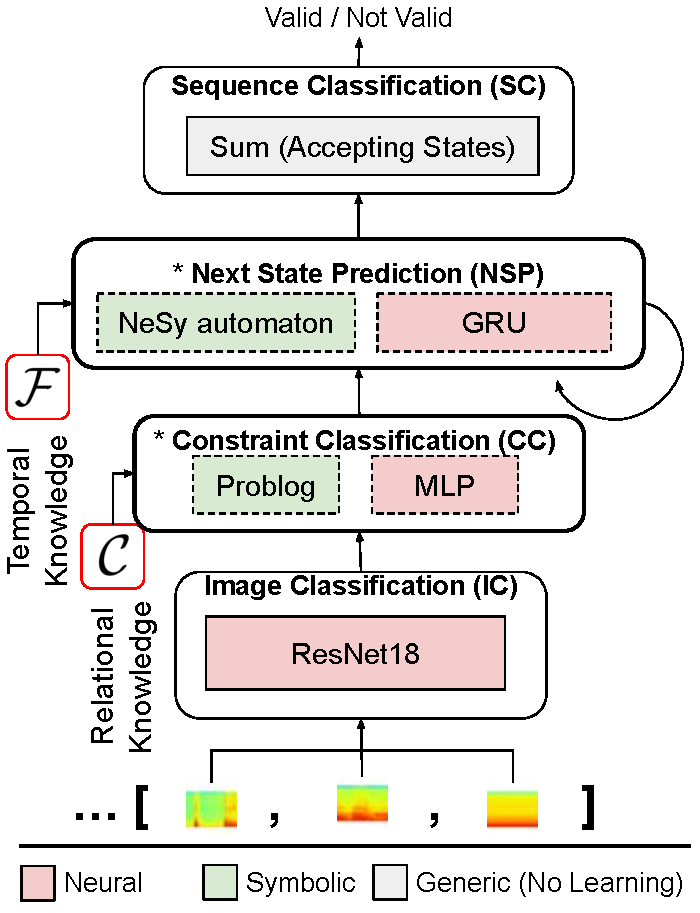
\includegraphics[width=0.5\linewidth]{imgs/ansya/Ansya Zinc.pdf}
\caption{Multi-stage architecture for temporal reasoning. Each block can be instantiated in either neural or symbolic flavors.}
\label{ansya:fig:arch}
\end{figure}
%TODO
\fi
\iffalse
We address the sequence classification task exemplified in Section~\ref{ansya:sec:case_study} by cascading multiple decisions, following the approach described in~\cite{lorello2025neuro}. In particular, we employ a multi-stage pipeline (Figure~\ref{ltlzinc:fig:pipeline}) composed of the following sub-tasks: ({\sc\small ic}) image classification, mapping data from each $\mathcal{X}_i$ to the corresponding $\mathcal{Y}_i$; ({\sc\small cc}) constraint classification, leveraging relational knowledge $\mathcal{C}$; ({\sc\small nsp}) next state prediction, leveraging temporal knowledge $\mathcal{F}$; ({\sc\small sc}) sequence classification, i.e., the final decision.
\fi
%
\iffalse
Formally, we are given a set of $N$ \textit{perceptual domains} (e.g., spectrograms) $\mathcal{X}_j, 0 \leq j < N$, each associated to a \textit{symbolic domain} $\mathcal{Y}_j$ (e.g., spectrogram categories).
%As an example, $\mathcal{X}_0$ and $\mathcal{X}_1$ could be the domains of MNIST digits and Fashion-MNIST articles~\cite{xiao2017fmnist}, respectively, whereas $\mathcal{Y}_0$ and $\mathcal{Y}_1$ the corresponding sets of (symbolic) classes. 
We indicate with $x_j^{t} \in \mathcal{X}_j$ and $y_j^{t} \in \mathcal{Y}_j$ a \textit{perceptual stimulus} and its \textit{symbolic label} observed at discrete time $0 \leq t < T$.
%
Let $\mathcal{C}$ be a \textit{mapping of relational constraints} from a string identifier to a predicate $\texttt{p/k}$ of arity $1 \leq k < N$ between symbolic labels; at each timestep $t$, the tuple of labels $\langle y^t_0, y^t_1, \dots, y^t_{N-1} \rangle$ corresponding to a certain stimulus $\langle x^t_0, x^t_1, \dots, x^t_{N-1} \rangle$ may or may not satisfy some predicates in $\mathcal{C}$. In this work, we consider constraints in $\mathcal{C}$ to have MiniZinc~\cite{nethercote2007minizinc} semantics.
%

Finally, let $\mathcal{F}$ be a \textit{temporal specification}, defined as an \LTLf formula over the set of relations in $\mathcal{C}$,  grounded with values in $\mathcal{Y}$.
LTLZinc~\cite{lorello2025neuro} %\footnote{%\url{https://anonymous.4open.science/r/LTLZinc-E9FF}
%\url{https://github.com/continual-nesy/LTLZinc}} 
is a benchmarking framework for temporal reasoning tasks, capable of generating sequences from user-defined constraint specifications involving relational and temporal knowledge. 
An LTLZinc problem is represented by the tuple $\langle \mathcal{X}, \mathcal{Y}, \mathcal{C}, \mathcal{F}\rangle$, instantiated over a finite time horizon $T$ as a collection of sequential observations. Such problem consists of a \textit{dataset of sequences}, composed of perceptual stimuli $\mathcal{S}_\mathcal{X} = ([x_0^t, \dots, x_{N-1}^t])_{t=0}^{T-1}$, and annotations: $\mathcal{S}_\mathcal{Y} = ([y_0^t, \dots, y_{N-1}^t])_{t=0}^{T-1}$ (symbolic label annotations), $\mathcal{S}_\mathcal{C} = ([c_0^t, \dots, c_{|\mathcal{C}|-1}^t])_{t=0}^{T-1}$ (constraint annotations, $c_i^t \in [\top, \bot]$), and $\mathcal{L} = [\top, \bot]$ (sequence label annotation, true if and only if the sequence satisfies $\mathcal{F}$). While the first three are sequential annotations, associated with each timestep of the input stimulus, the last one is a single value associated with the entire sequence.

The four stages are combined into: 
$P(f(\mathcal{S}) = 1) =  \left( \prod\limits_{t=0}^{T-1} P^t_{\text{\sc\tiny ic}} P^t_{\text{\sc\tiny cc}} P^t_{\text{\sc\tiny nsp}} \right) P_{\text{sc}}(f(\mathcal{S}) = 1 \mid \alpha^{T-1})$,
%\end{equation}
where $P^t_{\bullet}$ is the shorthand notation for the already introduced probabilities with arguments at time $t$.
We train our multi-stage architectures with four loss functions, each weighted by a $\lambda_{\bullet}$ hyper-parameter. \textsc{ic} and \textsc{nsp} (the latter conditioned on the previous state) exploit a %modules are both subjected to a 
categorical cross-entropy loss, %and weighted by $\lambda_{ic}$ and $\lambda_{ns}$, respectively. 
while \textsc{cc} and \textsc{sc} %are evaluated against 
a binary cross-entropy loss.
\fi
\iffalse
Each stage~$i$ is associated with a loss function, weighted by a corresponding hyper-parameter $\lambda_{i}$. 
%The LTLZinc framework provides annotations for each stage, which can be effectively disabled by fixing the corresponding lambda to zero.
\textsc{IC} and \textsc{NSP} are trained by means of categorical cross-entropy, while \textsc{CC} and \textsc{SC} employ a binary cross-entropy loss. %To stabilize training, we allow the \textsc{IC} module to be pre-trained to achieve good initial classification performance.


\section{Experiments}\label{ansya:sec:experiments}
Using the LTLZinc framework,\footnote{\url{https://github.com/continual-nesy/LTLZinc}} we generate three tasks, following well-known \LTL patterns for safety-critical applications~\cite{dwyer1998property}. For each task, we assume three spectrogram images $X, Y, Z$, %observed simultaneously at discrete timesteps, 
and the following constraint mapping $\mathcal{C}$:
\begin{align*}
\mathcal{C}\colon\quad&\texttt{p}(X, Y, Z): (X+Y) \equiv Z \mod 10;\\
&\texttt{q}(X, Y, Z): \texttt{all\_different}([X, Y, Z]);\\
&\texttt{r}(X, Y, Z): (X < Y < Z) \vee (X > Y > Z);\\
&\texttt{s}(X, Y, Z): X \not =  Z \wedge (X = Y \vee Y = Z).
\end{align*}
Each task corresponds to a different safety-critical property $\mathcal{F}$:
\begin{description}
\item[\textsc{Immediate Failure}] \texttt{p} is false after \texttt{r}:\\ $\ltlglobally (\texttt{r} \rightarrow \ltlglobally \neg \texttt{p})$;
\item[\textsc{Liveness}] \texttt{s} always follows \texttt{p}:\\ $\ltlglobally (\texttt{p} \rightarrow \ltlfinally \texttt{s})$;
\item[\textsc{Real-Time Response}] \texttt{s} responds to \texttt{p} between \texttt{q} and \texttt{r}:\\ $\ltlglobally ((\texttt{q} \wedge \ltlnext \ltlfinally \texttt{r}) \rightarrow (\texttt{p} \rightarrow (\neg \texttt{r} \ltluntil (\texttt{s} \wedge \neg \texttt{r}))) \ltluntil \texttt{r})$.
\end{description}
%
Datasets contain 1000 sequences (800 train, 100 validation, 100 test samples) of random length between 10 and 25 timesteps. Each timestep is associated with three RGB images sampled from the UrbanSound-Spectrogram dataset,\footnote{\url{https://github.com/mashrin/UrbanSound-Spectrogram}.} resized to fit into an $224\times 224$ image with white background. Images are augmented during training and inference, according to the original ResNet18 transforms~\cite{he2016deep}.
%
The  modular architecture of Figure ~\ref{ltlzinc:fig:pipeline} is initialized in two flavors: \textsc{Neural} (ResNet18, MLP, GRU, red dashed blocks), and \textsc{NeSy} (ResNet18, Deep Problog~\cite{manhaeve2019deepproblog}, NeSy Automaton~\cite{umili2023grounding}, green dashed blocks).
After selecting optimal hyper-parameters (optimizer: Adam, learning rate: $10^{-4}$, MLP:  64 neurons, GRU: 64 hidden units) on a simplified task (the one introduced in Sec.~\ref{ansya:sec:case_study}), we initialize the \textsc{IC} module with one epoch of pre-training on image labels only, then provide supervisions at every stage ($\lambda_{\textsc{CC}} = \lambda_{\textsc{NSP}} = \lambda_{\textsc{SC}} = 1.0, \lambda_\textsc{IC} = 0.1$) for a maximum of 7 epochs. 


Table~\ref{ansya:tab:results} summarizes the results on the test set, evaluated on the best-performing epoch (selected by average accuracy across all modules, measured on the validation set). In general, it can be observed that, although both \textsc{Neural} and \textsc{NeSy} methods reach similar image classification performance, downstream objectives become increasingly difficult for the Neural-only method. Overall, the \textsc{NeSy} method achieves the best performance across all symbolic objectives for every task, even though there is margin for improvement. Knowledge availability can only partially compensate the challenging nature of this setting, as even \textsc{NeSy} approaches struggle with harder formulae. Training behavior (not shown)  indicates that this effect is caused by severe over-fitting at the \textsc{NSP} stage, in spite of good upstream generalization of the \textsc{CC} objective, highlighting optimization challenges of the NeSy Automaton module, in spite of full supervisions available.









\fi
\iffalse

\begin{table*}[!t]
\centering
%\resizebox{\textwidth}{!}{
	\begin{tabular}{ccccccccccc}
		\toprule
		Task & Category & Best epoch & Learning rate & $\lambda_{IC}$ & $\lambda_{CC}$ & Avg acc $\uparrow$ & Label acc $\uparrow$ & Constraint acc $\uparrow$ & Successor acc $\uparrow$ & Sequence Acc $\uparrow$\\
		\midrule
		\multirow{2}{*}{Task 1} & Symbolic & $6$ & $1 \cdot 10^{-4}$ & $0.0$ & $1.0$ & $\textbf{0.88} $ {\tiny ($\pm 0.03$)} & $\textbf{0.82} $ {\tiny ($\pm 0.02$)} & $\textbf{0.95} $ {\tiny ($\pm 0.01$)} & $\textbf{0.89} $ {\tiny ($\pm 0.04$)} & $\textbf{0.87} $ {\tiny ($\pm 0.05$)}\\
		& Neural & $6$ & $1 \cdot 10^{-4}$ & $1.0$ & $1.0$ & $0.87 $ {\tiny ($\pm 0.04$)} & $0.81 $ {\tiny ($\pm 0.03$)} & $0.93 $ {\tiny ($\pm 0.01$)} & $0.85 $ {\tiny ($\pm 0.06$)} & $\textbf{0.87} $ {\tiny ($\pm 0.06$)}\\
		\midrule
		\multirow{2}{*}{Task 2} & Symbolic & $9$ & $1 \cdot 10^{-4}$ & $0.0$ & $0.0$ & $0.83 $ {\tiny ($\pm 0.03$)} & $0.76 $ {\tiny ($\pm 0.05$)} & $0.92 $ {\tiny ($\pm 0.02$)} & $0.80 $ {\tiny ($\pm 0.03$)} & $0.84 $ {\tiny ($\pm 0.04$)}\\
		& Neural & $6$ & $1 \cdot 10^{-4}$ & $1.0$ & $1.0$ & $\textbf{0.87} $ {\tiny ($\pm 0.02$)} & $\textbf{0.82} $ {\tiny ($\pm 0.02$)} & $\textbf{0.94} $ {\tiny ($\pm 0.01$)} & $\textbf{0.87} $ {\tiny ($\pm 0.03$)} & $\textbf{0.87} $ {\tiny ($\pm 0.05$)}\\
		\midrule
		\multirow{2}{*}{Task 3} & Symbolic & $0$ & $1 \cdot 10^{-3}$ & $1.0$ & $0.0$ & $\textbf{0.78} $ {\tiny ($\pm 0.03$)} & $\textbf{0.78} $ {\tiny ($\pm 0.04$)} & $\textbf{0.90} $ {\tiny ($\pm 0.03$)} & $\textbf{0.70} $ {\tiny ($\pm 0.04$)} & $0.75 $ {\tiny ($\pm 0.04$)}\\
		& Neural & $7$ & $1 \cdot 10^{-4}$ & $1.0$ & $0.0$ & $0.75 $ {\tiny ($\pm 0.09$)} & $0.74 $ {\tiny ($\pm 0.07$)} & $0.82 $ {\tiny ($\pm 0.01$)} & $0.66 $ {\tiny ($\pm 0.19$)} & $\textbf{0.79} $ {\tiny ($\pm 0.10$)}\\
		
		\bottomrule
	\end{tabular}
	%}
\caption{TODO: Epoch 0 = only pre-training.}
\end{table*}

\begin{table*}[!t]
\centering
%\resizebox{\textwidth}{!}{
	\begin{tabular}{ccccccccc}
		\toprule
		Expressivity & Pattern & Category & Best epoch & Avg accuracy $\uparrow$ & Label accuracy $\uparrow$ & Constraint accuracy $\uparrow$ & Successor accuracy $\uparrow$ & Sequence Accuracy $\uparrow$\\
		\midrule
		\multirow{19}{*}{\rotatebox[origin=c]{90}{FOL}} & \multirow{2}{*}{P1} & Symbolic & $0$ & $\textbf{0.68} $ {\tiny ($\pm 0.01$)} & $\textbf{0.77} $ {\tiny ($\pm 0.02$)} & $\textbf{0.85} $ {\tiny ($\pm 0.01$)} & $\textbf{0.56} $ {\tiny ($\pm 0.02$)} & $\textbf{0.56} $ {\tiny ($\pm 0.01$)}\\
		&  & Neural & $1$ & $0.62 $ {\tiny ($\pm 0.01$)} & $0.75 $ {\tiny ($\pm 0.02$)} & $0.78 $ {\tiny ($\pm 0.01$)} & $0.46 $ {\tiny ($\pm 0.00$)} & $0.50 $ {\tiny ($\pm 0.00$)}\\
		\cmidrule{2-9}
		& \multirow{2}{*}{P2} & Symbolic & $0$ & $\textbf{0.70} $ {\tiny ($\pm 0.01$)} & $\textbf{0.76} $ {\tiny ($\pm 0.01$)} & $\textbf{0.86} $ {\tiny ($\pm 0.00$)} & $\textbf{0.60} $ {\tiny ($\pm 0.02$)} & $\textbf{0.58} $ {\tiny ($\pm 0.03$)}\\
		&  & Neural & $1$ & $0.65 $ {\tiny ($\pm 0.02$)} & $0.75 $ {\tiny ($\pm 0.01$)} & $0.85 $ {\tiny ($\pm 0.01$)} & $0.52 $ {\tiny ($\pm 0.07$)} & $0.50 $ {\tiny ($\pm 0.00$)}\\
		\cmidrule{2-9}
		& \multirow{2}{*}{P3} & Symbolic & $0$ & $\textbf{0.64} $ {\tiny ($\pm 0.01$)} & $\textbf{0.77} $ {\tiny ($\pm 0.00$)} & $\textbf{0.86} $ {\tiny ($\pm 0.00$)} & $0.36 $ {\tiny ($\pm 0.01$)} & $\textbf{0.58} $ {\tiny ($\pm 0.04$)}\\
		&  & Neural & $1$ & $\textbf{0.64} $ {\tiny ($\pm 0.04$)} & $0.74 $ {\tiny ($\pm 0.00$)} & $0.81 $ {\tiny ($\pm 0.01$)} & $\textbf{0.54} $ {\tiny ($\pm 0.12$)} & $0.48 $ {\tiny ($\pm 0.03$)}\\
		\cmidrule{2-9}
		& \multirow{2}{*}{P4} & Symbolic & $0$ & $\textbf{0.68} $ {\tiny ($\pm 0.01$)} & $\textbf{0.77} $ {\tiny ($\pm 0.01$)} & $\textbf{0.85} $ {\tiny ($\pm 0.00$)} & $\textbf{0.57} $ {\tiny ($\pm 0.03$)} & $\textbf{0.52} $ {\tiny ($\pm 0.03$)}\\
		&  & Neural & $1$ & $0.61 $ {\tiny ($\pm 0.01$)} & $0.74 $ {\tiny ($\pm 0.02$)} & $0.80 $ {\tiny ($\pm 0.00$)} & $0.39 $ {\tiny ($\pm 0.05$)} & $0.50 $ {\tiny ($\pm 0.00$)}\\
		\cmidrule{2-9}
		& \multirow{2}{*}{P5} & Symbolic & $0$ & $\textbf{0.74} $ {\tiny ($\pm 0.01$)} & $\textbf{0.77} $ {\tiny ($\pm 0.01$)} & $\textbf{0.82} $ {\tiny ($\pm 0.01$)} & $\textbf{0.67} $ {\tiny ($\pm 0.01$)} & $\textbf{0.71} $ {\tiny ($\pm 0.03$)}\\
		&  & Neural & $1$ & $0.62 $ {\tiny ($\pm 0.03$)} & $0.60 $ {\tiny ($\pm 0.07$)} & $0.70 $ {\tiny ($\pm 0.01$)} & $0.57 $ {\tiny ($\pm 0.06$)} & $0.60 $ {\tiny ($\pm 0.04$)}\\
		\cmidrule{2-9}
		& \multirow{2}{*}{P6} & Symbolic & $0$ & $\textbf{0.68} $ {\tiny ($\pm 0.01$)} & $0.73 $ {\tiny ($\pm 0.01$)} & $\textbf{0.83} $ {\tiny ($\pm 0.00$)} & $\textbf{0.57} $ {\tiny ($\pm 0.03$)} & $\textbf{0.57} $ {\tiny ($\pm 0.02$)}\\
		&  & Neural & $1$ & $0.61 $ {\tiny ($\pm 0.05$)} & $\textbf{0.75} $ {\tiny ($\pm 0.03$)} & $0.81 $ {\tiny ($\pm 0.01$)} & $0.37 $ {\tiny ($\pm 0.19$)} & $0.50 $ {\tiny ($\pm 0.00$)}\\
		\cmidrule{2-9}
		& \multirow{2}{*}{P7} & Symbolic & $0$ & $\textbf{0.73} $ {\tiny ($\pm 0.01$)} & $\textbf{0.78} $ {\tiny ($\pm 0.01$)} & $\textbf{0.81} $ {\tiny ($\pm 0.00$)} & $\textbf{0.66} $ {\tiny ($\pm 0.01$)} & $\textbf{0.69} $ {\tiny ($\pm 0.03$)}\\
		&  & Neural & $1$ & $0.66 $ {\tiny ($\pm 0.02$)} & $0.69 $ {\tiny ($\pm 0.03$)} & $0.69 $ {\tiny ($\pm 0.03$)} & $0.59 $ {\tiny ($\pm 0.01$)} & $0.65 $ {\tiny ($\pm 0.05$)}\\
		\cmidrule{2-9}
		& \multirow{2}{*}{P8} & Symbolic & $0$ & $\textbf{0.65} $ {\tiny ($\pm 0.02$)} & $\textbf{0.77} $ {\tiny ($\pm 0.02$)} & $\textbf{0.83} $ {\tiny ($\pm 0.01$)} & $\textbf{0.47} $ {\tiny ($\pm 0.01$)} & $\textbf{0.55} $ {\tiny ($\pm 0.05$)}\\
		&  & Neural & $1$ & $0.57 $ {\tiny ($\pm 0.03$)} & $0.72 $ {\tiny ($\pm 0.03$)} & $0.75 $ {\tiny ($\pm 0.01$)} & $0.31 $ {\tiny ($\pm 0.08$)} & $0.50 $ {\tiny ($\pm 0.00$)}\\
		\cmidrule{2-9}
		& \multirow{2}{*}{P9} & Symbolic & $0$ & $\textbf{0.65} $ {\tiny ($\pm 0.04$)} & $\textbf{0.76} $ {\tiny ($\pm 0.05$)} & $\textbf{0.83} $ {\tiny ($\pm 0.03$)} & $\textbf{0.47} $ {\tiny ($\pm 0.04$)} & $0.56 $ {\tiny ($\pm 0.04$)}\\
		&  & Neural & $1$ & $0.62 $ {\tiny ($\pm 0.01$)} & $0.71 $ {\tiny ($\pm 0.05$)} & $0.76 $ {\tiny ($\pm 0.02$)} & $0.43 $ {\tiny ($\pm 0.00$)} & $\textbf{0.59} $ {\tiny ($\pm 0.02$)}\\
		\bottomrule\toprule
		\multirow{19}{*}{\rotatebox[origin=c]{90}{Propositional}} & \multirow{2}{*}{P1} & Symbolic & $0$ & $\textbf{0.67} $ {\tiny ($\pm 0.03$)} & $\textbf{0.72} $ {\tiny ($\pm 0.02$)} & $\textbf{0.82} $ {\tiny ($\pm 0.02$)} & $\textbf{0.58} $ {\tiny ($\pm 0.05$)} & $\textbf{0.55} $ {\tiny ($\pm 0.06$)}\\
		&  & Neural & $1$ & $0.61 $ {\tiny ($\pm 0.00$)} & $0.69 $ {\tiny ($\pm 0.02$)} & $0.78 $ {\tiny ($\pm 0.02$)} & $0.44 $ {\tiny ($\pm 0.00$)} & $0.52 $ {\tiny ($\pm 0.05$)}\\
		\cmidrule{2-9}
		& \multirow{2}{*}{P2} & Symbolic & $0$ & $\textbf{0.65} $ {\tiny ($\pm 0.03$)} & $\textbf{0.70} $ {\tiny ($\pm 0.05$)} & $\textbf{0.81} $ {\tiny ($\pm 0.05$)} & $0.57 $ {\tiny ($\pm 0.03$)} & $0.51 $ {\tiny ($\pm 0.01$)}\\
		&  & Neural & $1$ & $\textbf{0.65} $ {\tiny ($\pm 0.05$)} & $0.62 $ {\tiny ($\pm 0.06$)} & $0.77 $ {\tiny ($\pm 0.04$)} & $\textbf{0.61} $ {\tiny ($\pm 0.10$)} & $\textbf{0.60} $ {\tiny ($\pm 0.09$)}\\
		\cmidrule{2-9}
		& \multirow{2}{*}{P3} & Symbolic & $0$ & $\textbf{0.62} $ {\tiny ($\pm 0.02$)} & $\textbf{0.62} $ {\tiny ($\pm 0.04$)} & $\textbf{0.77} $ {\tiny ($\pm 0.02$)} & $\textbf{0.57} $ {\tiny ($\pm 0.02$)} & $\textbf{0.51} $ {\tiny ($\pm 0.01$)}\\
		&  & Neural & $1$ & $0.54 $ {\tiny ($\pm 0.05$)} & $0.61 $ {\tiny ($\pm 0.08$)} & $\textbf{0.77} $ {\tiny ($\pm 0.07$)} & $0.31 $ {\tiny ($\pm 0.08$)} & $0.48 $ {\tiny ($\pm 0.06$)}\\
		\cmidrule{2-9}
		& \multirow{2}{*}{P4} & Symbolic & $0$ & $\textbf{0.61} $ {\tiny ($\pm 0.02$)} & $\textbf{0.67} $ {\tiny ($\pm 0.04$)} & $\textbf{0.79} $ {\tiny ($\pm 0.03$)} & $0.47 $ {\tiny ($\pm 0.02$)} & $0.49 $ {\tiny ($\pm 0.01$)}\\
		&  & Neural & $1$ & $\textbf{0.61} $ {\tiny ($\pm 0.02$)} & $0.63 $ {\tiny ($\pm 0.03$)} & $0.78 $ {\tiny ($\pm 0.01$)} & $\textbf{0.53} $ {\tiny ($\pm 0.04$)} & $\textbf{0.52} $ {\tiny ($\pm 0.06$)}\\
		\cmidrule{2-9}
		& \multirow{2}{*}{P5} & Symbolic & $0$ & $\textbf{0.74} $ {\tiny ($\pm 0.03$)} & $\textbf{0.69} $ {\tiny ($\pm 0.04$)} & $\textbf{0.79} $ {\tiny ($\pm 0.02$)} & $\textbf{0.74} $ {\tiny ($\pm 0.01$)} & $\textbf{0.75} $ {\tiny ($\pm 0.04$)}\\
		&  & Neural & $1$ & $0.71 $ {\tiny ($\pm 0.05$)} & $0.60 $ {\tiny ($\pm 0.06$)} & $0.77 $ {\tiny ($\pm 0.04$)} & $0.73 $ {\tiny ($\pm 0.05$)} & $0.74 $ {\tiny ($\pm 0.07$)}\\
		\cmidrule{2-9}
		& \multirow{2}{*}{P6} & Symbolic & $0$ & $\textbf{0.69} $ {\tiny ($\pm 0.06$)} & $\textbf{0.68} $ {\tiny ($\pm 0.04$)} & $0.80 $ {\tiny ($\pm 0.03$)} & $\textbf{0.64} $ {\tiny ($\pm 0.08$)} & $\textbf{0.67} $ {\tiny ($\pm 0.10$)}\\
		&  & Neural & $1$ & $0.62 $ {\tiny ($\pm 0.02$)} & $0.67 $ {\tiny ($\pm 0.05$)} & $\textbf{0.82} $ {\tiny ($\pm 0.02$)} & $0.49 $ {\tiny ($\pm 0.02$)} & $0.50 $ {\tiny ($\pm 0.03$)}\\
		\cmidrule{2-9}
		& \multirow{2}{*}{P7} & Symbolic & $0$ & $\textbf{0.75} $ {\tiny ($\pm 0.02$)} & $\textbf{0.68} $ {\tiny ($\pm 0.04$)} & $\textbf{0.82} $ {\tiny ($\pm 0.01$)} & $\textbf{0.75} $ {\tiny ($\pm 0.02$)} & $\textbf{0.75} $ {\tiny ($\pm 0.02$)}\\
		&  & Neural & $1$ & $0.69 $ {\tiny ($\pm 0.03$)} & $0.59 $ {\tiny ($\pm 0.03$)} & $0.78 $ {\tiny ($\pm 0.03$)} & $0.72 $ {\tiny ($\pm 0.02$)} & $0.70 $ {\tiny ($\pm 0.06$)}\\
		\cmidrule{2-9}
		& \multirow{2}{*}{P8} & Symbolic & $0$ & $0.61 $ {\tiny ($\pm 0.02$)} & $\textbf{0.64} $ {\tiny ($\pm 0.03$)} & $0.78 $ {\tiny ($\pm 0.05$)} & $0.47 $ {\tiny ($\pm 0.02$)} & $0.54 $ {\tiny ($\pm 0.01$)}\\
		&  & Neural & $1$ & $\textbf{0.67} $ {\tiny ($\pm 0.01$)} & $\textbf{0.64} $ {\tiny ($\pm 0.02$)} & $\textbf{0.79} $ {\tiny ($\pm 0.02$)} & $\textbf{0.54} $ {\tiny ($\pm 0.02$)} & $\textbf{0.70} $ {\tiny ($\pm 0.02$)}\\
		\cmidrule{2-9}
		& \multirow{2}{*}{P9} & Symbolic & $0$ & $0.63 $ {\tiny ($\pm 0.04$)} & $\textbf{0.68} $ {\tiny ($\pm 0.03$)} & $\textbf{0.82} $ {\tiny ($\pm 0.01$)} & $0.48 $ {\tiny ($\pm 0.07$)} & $0.56 $ {\tiny ($\pm 0.04$)}\\
		&  & Neural & $1$ & $\textbf{0.67} $ {\tiny ($\pm 0.01$)} & $0.59 $ {\tiny ($\pm 0.01$)} & $0.79 $ {\tiny ($\pm 0.02$)} & $\textbf{0.57} $ {\tiny ($\pm 0.01$)} & $\textbf{0.71} $ {\tiny ($\pm 0.01$)}\\
		
		\bottomrule
	\end{tabular}
	%}
\caption{TODO: 1 pre-training epoch + 1 full training epoch. Best epoch 0 = only pre-training.}
\end{table*}

\begin{table*}[!t]
\centering
%\resizebox{\textwidth}{!}{
	\begin{tabular}{ccccccccc}
		\toprule
		Expressivity & Pattern & Category & Best epoch & Avg accuracy $\uparrow$ & Label accuracy $\uparrow$ & Constraint accuracy $\uparrow$ & Successor accuracy $\uparrow$ & Sequence Accuracy $\uparrow$\\
		\midrule
		\multirow{19}{*}{\rotatebox[origin=c]{90}{FOL}} & \multirow{2}{*}{P1} & Symbolic & $1$ & $\textbf{0.70} $ {\tiny ($\pm 0.02$)} & $\textbf{0.79} $ {\tiny ($\pm 0.02$)} & $\textbf{0.86} $ {\tiny ($\pm 0.01$)} & $\textbf{0.57} $ {\tiny ($\pm 0.03$)} & $\textbf{0.59} $ {\tiny ($\pm 0.03$)}\\
		& & Neural & $5$ & $0.63 $ {\tiny ($\pm 0.00$)} & $0.78 $ {\tiny ($\pm 0.02$)} & $0.78 $ {\tiny ($\pm 0.01$)} & $0.46 $ {\tiny ($\pm 0.00$)} & $0.50 $ {\tiny ($\pm 0.01$)}\\
		\cmidrule{2-9}
		& \multirow{2}{*}{P2} & Symbolic & $5$ & $\textbf{0.73} $ {\tiny ($\pm 0.04$)} & $0.78 $ {\tiny ($\pm 0.04$)} & $\textbf{0.87} $ {\tiny ($\pm 0.02$)} & $\textbf{0.63} $ {\tiny ($\pm 0.05$)} & $\textbf{0.63} $ {\tiny ($\pm 0.05$)}\\
		& & Neural & $5$ & $0.68 $ {\tiny ($\pm 0.00$)} & $\textbf{0.80} $ {\tiny ($\pm 0.01$)} & $0.86 $ {\tiny ($\pm 0.01$)} & $0.57 $ {\tiny ($\pm 0.00$)} & $0.50 $ {\tiny ($\pm 0.00$)}\\
		\cmidrule{2-9}
		& \multirow{2}{*}{P3} & Symbolic & $7$ & $\textbf{0.68} $ {\tiny ($\pm 0.01$)} & $\textbf{0.80} $ {\tiny ($\pm 0.02$)} & $\textbf{0.87} $ {\tiny ($\pm 0.01$)} & $0.46 $ {\tiny ($\pm 0.04$)} & $\textbf{0.58} $ {\tiny ($\pm 0.02$)}\\
		&  & Neural & $6$ & $\textbf{0.68} $ {\tiny ($\pm 0.01$)} & $\textbf{0.80} $ {\tiny ($\pm 0.01$)} & $0.81 $ {\tiny ($\pm 0.01$)} & $\textbf{0.61} $ {\tiny ($\pm 0.00$)} & $0.50 $ {\tiny ($\pm 0.00$)}\\
		\cmidrule{2-9}
		& \multirow{2}{*}{P4} & Symbolic & $7$ & $\textbf{0.70} $ {\tiny ($\pm 0.02$)} & $\textbf{0.80} $ {\tiny ($\pm 0.02$)} & $\textbf{0.85} $ {\tiny ($\pm 0.01$)} & $\textbf{0.59} $ {\tiny ($\pm 0.02$)} & $\textbf{0.57} $ {\tiny ($\pm 0.04$)}\\
		&  & Neural & $7$ & $0.61 $ {\tiny ($\pm 0.02$)} & $0.78 $ {\tiny ($\pm 0.01$)} & $0.80 $ {\tiny ($\pm 0.01$)} & $0.38 $ {\tiny ($\pm 0.07$)} & $0.50 $ {\tiny ($\pm 0.00$)}\\
		\cmidrule{2-9}
		& \multirow{2}{*}{P5} & Symbolic & $2$ & $\textbf{0.76} $ {\tiny ($\pm 0.01$)} & $\textbf{0.80} $ {\tiny ($\pm 0.01$)} & $\textbf{0.83} $ {\tiny ($\pm 0.01$)} & $\textbf{0.69} $ {\tiny ($\pm 0.00$)} & $\textbf{0.71} $ {\tiny ($\pm 0.01$)}\\
		&  & Neural & $5$ & $0.68 $ {\tiny ($\pm 0.01$)} & $0.76 $ {\tiny ($\pm 0.02$)} & $0.72 $ {\tiny ($\pm 0.01$)} & $0.64 $ {\tiny ($\pm 0.01$)} & $0.59 $ {\tiny ($\pm 0.02$)}\\
		\cmidrule{2-9}
		& \multirow{2}{*}{P6} & Symbolic & $3$ & $\textbf{0.73} $ {\tiny ($\pm 0.01$)} & $\textbf{0.79} $ {\tiny ($\pm 0.02$)} & $\textbf{0.87} $ {\tiny ($\pm 0.01$)} & $\textbf{0.64} $ {\tiny ($\pm 0.02$)} & $\textbf{0.60} $ {\tiny ($\pm 0.03$)}\\
		&  & Neural & $6$ & $0.64 $ {\tiny ($\pm 0.01$)} & $\textbf{0.79} $ {\tiny ($\pm 0.02$)} & $0.81 $ {\tiny ($\pm 0.01$)} & $0.47 $ {\tiny ($\pm 0.00$)} & $0.50 $ {\tiny ($\pm 0.00$)}\\
		\cmidrule{2-9}
		& \multirow{2}{*}{P7} & Symbolic & $3$ & $\textbf{0.76} $ {\tiny ($\pm 0.02$)} & $\textbf{0.81} $ {\tiny ($\pm 0.02$)} & $\textbf{0.83} $ {\tiny ($\pm 0.02$)} & $\textbf{0.68} $ {\tiny ($\pm 0.02$)} & $\textbf{0.71} $ {\tiny ($\pm 0.03$)}\\
		&  & Neural & $7$ & $0.71 $ {\tiny ($\pm 0.01$)} & $0.78 $ {\tiny ($\pm 0.00$)} & $0.72 $ {\tiny ($\pm 0.01$)} & $0.63 $ {\tiny ($\pm 0.01$)} & $0.70 $ {\tiny ($\pm 0.05$)}\\
		\cmidrule{2-9}
		& \multirow{2}{*}{P8} & Symbolic & $3$ & $\textbf{0.66} $ {\tiny ($\pm 0.02$)} & $\textbf{0.80} $ {\tiny ($\pm 0.00$)} & $\textbf{0.85} $ {\tiny ($\pm 0.01$)} & $\textbf{0.48} $ {\tiny ($\pm 0.00$)} & $\textbf{0.52} $ {\tiny ($\pm 0.07$)}\\
		&  & Neural & $6$ & $0.59 $ {\tiny ($\pm 0.02$)} & $0.76 $ {\tiny ($\pm 0.06$)} & $0.76 $ {\tiny ($\pm 0.02$)} & $0.35 $ {\tiny ($\pm 0.02$)} & $0.50 $ {\tiny ($\pm 0.00$)}\\
		\cmidrule{2-9}
		& \multirow{2}{*}{P9} & Symbolic & $4$ & $\textbf{0.68} $ {\tiny ($\pm 0.02$)} & $\textbf{0.78} $ {\tiny ($\pm 0.03$)} & $\textbf{0.84} $ {\tiny ($\pm 0.01$)} & $\textbf{0.49} $ {\tiny ($\pm 0.02$)} & $0.60 $ {\tiny ($\pm 0.02$)}\\
		&  & Neural & $6$ & $0.66 $ {\tiny ($\pm 0.00$)} & $\textbf{0.78} $ {\tiny ($\pm 0.02$)} & $0.76 $ {\tiny ($\pm 0.01$)} & $0.45 $ {\tiny ($\pm 0.00$)} & $\textbf{0.63} $ {\tiny ($\pm 0.02$)}\\
		\bottomrule\toprule
		\multirow{19}{*}{\rotatebox[origin=c]{90}{Propositional}} & \multirow{2}{*}{P1} & Symbolic & $1$ & $\textbf{0.71} $ {\tiny ($\pm 0.04$)} & $\textbf{0.74} $ {\tiny ($\pm 0.02$)} & $\textbf{0.84} $ {\tiny ($\pm 0.01$)} & $\textbf{0.65} $ {\tiny ($\pm 0.06$)} & $0.60 $ {\tiny ($\pm 0.05$)}\\
		&  & Neural & $7$ & $0.69 $ {\tiny ($\pm 0.02$)} & $0.72 $ {\tiny ($\pm 0.05$)} & $0.83 $ {\tiny ($\pm 0.03$)} & $0.54 $ {\tiny ($\pm 0.02$)} & $\textbf{0.65} $ {\tiny ($\pm 0.03$)}\\
		\cmidrule{2-9}
		& \multirow{2}{*}{P2} & Symbolic & $5$ & $0.67 $ {\tiny ($\pm 0.03$)} & $\textbf{0.73} $ {\tiny ($\pm 0.05$)} & $\textbf{0.83} $ {\tiny ($\pm 0.03$)} & $0.60 $ {\tiny ($\pm 0.04$)} & $0.53 $ {\tiny ($\pm 0.01$)}\\
		&  & Neural & $5$ & $\textbf{0.70} $ {\tiny ($\pm 0.08$)} & $0.70 $ {\tiny ($\pm 0.08$)} & $0.81 $ {\tiny ($\pm 0.05$)} & $\textbf{0.67} $ {\tiny ($\pm 0.08$)} & $\textbf{0.64} $ {\tiny ($\pm 0.12$)}\\
		\cmidrule{2-9}
		& \multirow{2}{*}{P3} & Symbolic & $0$ & $\textbf{0.63} $ {\tiny ($\pm 0.02$)} & $0.63 $ {\tiny ($\pm 0.05$)} & $0.78 $ {\tiny ($\pm 0.03$)} & $\textbf{0.58} $ {\tiny ($\pm 0.01$)} & $\textbf{0.52} $ {\tiny ($\pm 0.01$)}\\
		&  & Neural & $6$ & $0.60 $ {\tiny ($\pm 0.01$)} & $\textbf{0.73} $ {\tiny ($\pm 0.01$)} & $\textbf{0.85} $ {\tiny ($\pm 0.01$)} & $0.35 $ {\tiny ($\pm 0.00$)} & $0.47 $ {\tiny ($\pm 0.06$)}\\
		\cmidrule{2-9}
		& \multirow{2}{*}{P4} & Symbolic & $3$ & $\textbf{0.67} $ {\tiny ($\pm 0.03$)} & $\textbf{0.73} $ {\tiny ($\pm 0.01$)} & $\textbf{0.83} $ {\tiny ($\pm 0.01$)} & $\textbf{0.56} $ {\tiny ($\pm 0.05$)} & $0.54 $ {\tiny ($\pm 0.03$)}\\
		&  & Neural & $7$ & $0.66 $ {\tiny ($\pm 0.03$)} & $0.69 $ {\tiny ($\pm 0.02$)} & $0.81 $ {\tiny ($\pm 0.02$)} & $0.54 $ {\tiny ($\pm 0.04$)} & $\textbf{0.58} $ {\tiny ($\pm 0.05$)}\\
		\cmidrule{2-9}
		& \multirow{2}{*}{P5} & Symbolic & $6$ & $0.78 $ {\tiny ($\pm 0.03$)} & $0.74 $ {\tiny ($\pm 0.03$)} & $0.82 $ {\tiny ($\pm 0.04$)} & $0.79 $ {\tiny ($\pm 0.04$)} & $0.78 $ {\tiny ($\pm 0.02$)}\\
		&  & Neural & $6$ & $\textbf{0.81} $ {\tiny ($\pm 0.03$)} & $\textbf{0.76} $ {\tiny ($\pm 0.05$)} & $\textbf{0.84} $ {\tiny ($\pm 0.03$)} & $\textbf{0.83} $ {\tiny ($\pm 0.03$)} & $\textbf{0.84} $ {\tiny ($\pm 0.03$)}\\
		\cmidrule{2-9}
		& \multirow{2}{*}{P6} & Symbolic & $6$ & $\textbf{0.75} $ {\tiny ($\pm 0.03$)} & $0.71 $ {\tiny ($\pm 0.03$)} & $0.84 $ {\tiny ($\pm 0.01$)} & $\textbf{0.72} $ {\tiny ($\pm 0.05$)} & $\textbf{0.74} $ {\tiny ($\pm 0.05$)}\\
		&  & Neural & $7$ & $0.66 $ {\tiny ($\pm 0.01$)} & $\textbf{0.73} $ {\tiny ($\pm 0.01$)} & $\textbf{0.85} $ {\tiny ($\pm 0.01$)} & $0.57 $ {\tiny ($\pm 0.05$)} & $0.51 $ {\tiny ($\pm 0.02$)}\\
		\cmidrule{2-9}
		& \multirow{2}{*}{P7} & Symbolic & $2$ & $\textbf{0.82} $ {\tiny ($\pm 0.02$)} & $0.75 $ {\tiny ($\pm 0.02$)} & $\textbf{0.86} $ {\tiny ($\pm 0.02$)} & $\textbf{0.82} $ {\tiny ($\pm 0.02$)} & $\textbf{0.84} $ {\tiny ($\pm 0.03$)}\\
		&  & Neural & $7$ & $0.81 $ {\tiny ($\pm 0.01$)} & $\textbf{0.76} $ {\tiny ($\pm 0.00$)} & $0.85 $ {\tiny ($\pm 0.02$)} & $0.81 $ {\tiny ($\pm 0.02$)} & $0.82 $ {\tiny ($\pm 0.01$)}\\
		\cmidrule{2-9}
		& \multirow{2}{*}{P8} & Symbolic & $2$ & $\textbf{0.72} $ {\tiny ($\pm 0.01$)} & $\textbf{0.75} $ {\tiny ($\pm 0.03$)} & $\textbf{0.85} $ {\tiny ($\pm 0.01$)} & $\textbf{0.61} $ {\tiny ($\pm 0.01$)} & $0.66 $ {\tiny ($\pm 0.01$)}\\
		&  & Neural & $7$ & $0.70 $ {\tiny ($\pm 0.02$)} & $0.71 $ {\tiny ($\pm 0.01$)} & $0.81 $ {\tiny ($\pm 0.01$)} & $0.60 $ {\tiny ($\pm 0.03$)} & $\textbf{0.70} $ {\tiny ($\pm 0.06$)}\\
		\cmidrule{2-9}
		& \multirow{2}{*}{P9} & Symbolic & $7$ & $0.70 $ {\tiny ($\pm 0.06$)} & $0.72 $ {\tiny ($\pm 0.04$)} & $\textbf{0.85} $ {\tiny ($\pm 0.03$)} & $0.58 $ {\tiny ($\pm 0.09$)} & $0.64 $ {\tiny ($\pm 0.09$)}\\
		&  & Neural & $6$ & $\textbf{0.74} $ {\tiny ($\pm 0.03$)} & $\textbf{0.73} $ {\tiny ($\pm 0.04$)} & $\textbf{0.85} $ {\tiny ($\pm 0.03$)} & $\textbf{0.65} $ {\tiny ($\pm 0.04$)} & $\textbf{0.74} $ {\tiny ($\pm 0.02$)}\\
		
		\bottomrule
	\end{tabular}
	%}
\caption{TODO: 1 pre-training epoch + 7 full training epochs. Best epoch 0 = only pre-training.}
\end{table*}

\fi
\iffalse
%\section{Conclusions}\label{ansya:sec:conclusions}
%In this work, we explored the application of NeSy AI for relational-temporal reasoning to safety-critical systems. 

These preliminary experiments show that, while significantly outperforming knowledge-agnostic, neural-only methods, in every explored task, and in spite of perfect knowledge availability, NeSy performance quickly degrades as temporal behavior increases in complexity. To successfully deploy NeSy temporal reasoners in safety-critical settings, it is crucial to boost their performance in a way which is not affected by temporal complexity, especially for real-world settings, where full supervisions are not available.
\fi